% !TeX encoding = UTF-8
% !TeX program = pdflatex
% !BIB program = biber

%%%%%%%%%%%%%%%%%%%%%%%%%%%%%%%%%%%%%%%%%%%%%%%%%%%%%%%%%%%%%%%%%%%%%%%%%%
%%% Basierend auf der Vorlage von									   %%%
%%% Michael Vierhauser, Institut fuer Wirtschaftsinformatik, Nov 2019  %%%
%%% und der Vorlage von Ali Varli, Oct 2019                            %%%
%%% Coversheet by: Andreas Neubauer, May 2016                          %%%    
%%%%%%%%%%%%%%%%%%%%%%%%%%%%%%%%%%%%%%%%%%%%%%%%%%%%%%%%%%%%%%%%%%%%%%%%%%
\documentclass[a4paper,11pt,oneside,onecolumn,openany]{memoir}
% !TeX root = MAIN.tex
% !TeX encoding = UTF-8

\usepackage{datetime}   % Date and time methods
\usepackage{url}		% URL-sensitive line breaks
\usepackage{graphicx}	% For loading graphic files
\usepackage{color}
\usepackage[usenames,dvipsnames,table,hyperref]{xcolor} % provides easy driver-independent access to several kinds of color tints
\usepackage{microtype}  % Small-scale typographic enhancements.
\usepackage{xspace}		% Define commands that appear not to eat spaces
\usepackage{todonotes}	% Marking things to do in a LaTeX document
\usepackage{flafter}	% floats always appear after their definition
\usepackage{placeins}	% useful, for example, to ensure all floats for a section appear before the next section
\usepackage{lipsum}		% Easy access to the Lorem Ipsum dummy text
\usepackage{verbatim}	% Reimplementation of and extensions to LaTeX verbatim
\usepackage{afterpage}	% Execute command after the next page break
\usepackage{wrapfig}	% Produces figures which text can flow around
\usepackage[font=small,labelfont=bf,format=hang]{caption}	% Customising captions in floating environments
\usepackage{geometry}	% page borders, ...

% Table packages
%\usepackage{booktabs}   % enhances the quality of tables
%\usepackage{tabularx}	% enhanced table
%\usepackage{ltxtable}	% tabularx over multiple pages
%\usepackage{longtable}	% table over multiple pages
%\usepackage{multirow}	% Create tabular cells spanning multiple rows
%\usepackage{array}		% Extending the array and tabular environments
%\usepackage{bigstrut}	% Struts for opening up tabular spacing\dfrac{num}{den}
%\usepackage{makecell}	% Tabular column heads and multilined cells

% Load packages to allow in- and output of non-ASCII characters.
\usepackage{lmodern}        % Use an extension of the original Computer Modern font to minimize the use of bitmapped letters.
\usepackage[T1]{fontenc}    % Determines font encoding of the output. Font packages have to be included before this line.
\usepackage[utf8]{inputenc} % Determines encoding of the input. All input files have to use UTF8 encoding.

% Some more packages
\usepackage{nag}        % Issues warnings when best practices in writing LaTeX documents are violated.
\usepackage{hyperref}   % Enables cross linking in the electronic document version. This package has to be included second to last.
% !TeX root = MAIN.tex
% !TeX encoding = UTF-8

%%%%%%%%%%%%%%%%%%%%%%%%%%%%%%%%%%%%%%%%%
%%% DOCUMENT CONFIGURAITON           %%%% 
%%%%%%%%%%%%%%%%%%%%%%%%%%%%%%%%%%%%%%%%%

%% Language (comment the appropriate line with a % sign)
\newif\ifeng
%\engtrue
\engfalse

%% Title of the thesis
\def\thesisTitle{Ein ASP-basierter Ansatz zur Lösung des Nurse Scheduling Problems mit Clingo}

%% choose type of work: 0 ... Dissertation
%%                      1 ... Diplomarbeit
%%                      2 ... Masterarbeit
%%                      3 ... Bachelorarbeit
\def\type{3}

%% enter the name of the student
\def\name{Rafetseder Tobias}

%% enter the name of the supervisor and first thesis examiner
%% for the german version you also have to enter the sex (male or female)
%% of the supervisor/examiners
\def\supervisor{o. Univ.-Prof. Dipl.-Ing. Dr. techn. Michael Schrefl}
\newif\ifsupvismale
\supvismaletrue %% supervisor is male
%\supvismalefalse && supervisor is female

% secondexaminer (only for dissertation!)
\def\secondexaminer{Name des zweiten Prüfers}
\newif\ifsecexmale
\secexmaletrue %% second examiner is male
%\secexmalefalse %% second examiner is female

% if there has been assistance by a further person uncomment the following line
% and enter the name.
\def\assist{Dipl.-Ing. Sebastian Windsperger}

%% choose bibliography style: numeric ... Numerisch
%%                            alphabetic ... Alphabetisch
%%                            apa ... APA
%%                            ieee ... IEEE
\def\bibstyleselection{apa}

% enter month year
% (the month when you brought it to the Prüfungs- und Anerkennungsservice)
\def\date{Juni \the\year}

%% enter name of degree (as stated in your curriculum)
\ifeng
	\def\degree{\ifcase\type Doctor of Social Sciences, Economics \& Business \or Magister \or Master of Science \or Bachelor Science \fi}
\else
	\def\degree{\ifcase\type Doktor der Sozial- und Wirtschaftswissenschaften \or Magister \or Master of Science \or Bachelor Science \fi}
\fi

%% enter the study (Studienrichtung, as stated in your curriculum)
\ifeng
	\def\study{Business Informatics}
\else
	\def\study{Wirtschaftsinformatik}
\fi

%% enter the name of the institute and load other language dependent packages
\ifeng
	\def\institute{Institute for Business \\ Informatics - Data \& \\Knowledge Engineering}
\else
	\def\institute{Institut für Wirtschafts-informatik - Data \& \\Knowledge Engineering}
\fi

%%%%%%%%%%%%%%%%%%%%%%%%%%%%%%%%%%%%%%%%%
%%% PACKAGE CONFIGURAITON            %%%% 
%%%%%%%%%%%%%%%%%%%%%%%%%%%%%%%%%%%%%%%%%
% no need to change something below here
\title{\thesisTitle}
\author{\name}
\hypersetup {
	pdftitle={\thesisTitle},
	pdfauthor={\name},
	colorlinks=true,
	linktoc=all,
	linkcolor=black,
	citecolor=black,
	filecolor=black,
	urlcolor=black
}
\urlstyle{sf}
\newcolumntype{H}[1]{>{\hsize=#1\hsize\arraybackslash}X} % relative width of table columns with type H
\renewcommand{\arraystretch}{1.5} 			% padding in tables
\renewcommand{\familydefault}{\sfdefault} 	% sans-serif font
\setlength{\parindent}{0pt} % Remove paragraph identation
\chapterstyle{ell}		% chapter styling http://ctan.math.utah.edu/ctan/tex-archive/info/latex-samples/MemoirChapStyles/MemoirChapStyles.pdf
\setsecnumdepth{subsection} % enumerate subsection

\ifeng
	\usepackage[british]{babel}
	\selectlanguage{british}
	\usepackage[babel,english=british]{csquotes}
\else
	\usepackage[ngerman]{babel}
	\selectlanguage{ngerman}
	\usepackage[babel,german=guillemets]{csquotes}
\fi

\usepackage[backend=biber,style=\bibstyleselection]{biblatex}
\bibliography{literature} % Change this file to set title, author, ...
% !TeX root = MAIN.tex
% !TeX encoding = UTF-8

\usepackage{listings}
\usepackage{inconsolata}
\usepackage{textcomp}

\definecolor{cblue}{rgb}{0.13,0.13,1}
\definecolor{cgreen}{rgb}{0,0.5,0}
\definecolor{cred}{rgb}{0.9,0,0}
\definecolor{cgrey}{rgb}{0.46,0.45,0.48}
\definecolor{corange}{rgb}{0.93, 0.53, 0.18}
\definecolor{cgreen2}{rgb}{0.0, 0.42, 0.24}
\definecolor{cbrown}{rgb}{0.59, 0.29, 0.0}

\lstdefinelanguage{drools}{
    morekeywords={
        true, false, null,
        lock-on-active, date-effective, date-expires, no-loop, auto-focus, activation-group, agenda-group,
        ruleflow-group, entry-point, duration, package, import, dialect, salience, enabled, attributes, rule,
        extend, when, then, template, query, declare, function, global, eval, not, in, or, and, exists, forall,
        accumulate, collect, from, action, reverse, result, end, over, init, for, while, insert, delete, update,
        if, else, new, import, instanceof, do, break, class
    },
    alsoletter={-},
    sensitive=false,
    morecomment=[l]{//},
    morecomment=[s]{/*}{*/},
    morestring=[b]"
}

\lstdefinelanguage{properties}{
    morekeywords={
        true, false, null
    },
    alsoletter={-},
    sensitive=false,
    morecomment=[l]{\#},
    morestring=[b]"
}

\lstdefinelanguage{sparql}{
  sensitive=true,
  morecomment=[l][\color{cgrey}]{\#},       % comments
  morecomment=[n][\color{cgreen2}]{<http}{>}, % uris
  morestring=[b][\color{cgreen}]{\"},  % strings
  alsoletter={-},
  % -------------------------- variables
  keywordsprefix=?,
  classoffset=0,
  keywordstyle=\color{cbrown},
  morekeywords={},
  % -------------------------- prefixes
  classoffset=1,
  keywordstyle=\color{corange},
  morekeywords={rdf,rdfs,xsd,inst,sim,qbx,ontolex,wordnet},
  % -------------------------- keywords
  classoffset=2,
  keywordstyle=\color{cblue},
  morekeywords={
    SELECT,CONSTRUCT,DESCRIBE,ASK,WHERE,FROM,NAMED,PREFIX,BASE,OPTIONAL,
    FILTER,GRAPH,LIMIT,OFFSET,SERVICE,UNION,EXISTS,NOT,BINDINGS,MINUS,a,
    BIND,IRI,CONCAT,STRUUID,INSERT,DISTINCT,AS,GROUP,ORDER,BY,DESC,isLiteral
  }
}

\lstdefinelanguage{json}{
    string=[s]{"}{"},
    stringstyle=\color{cblue},
    comment=[l]{:},
    commentstyle=\color{black},
    literate=
        *{0}{{{\color{numb}0}}}{1}
         {1}{{{\color{numb}1}}}{1}
         {2}{{{\color{numb}2}}}{1}
         {3}{{{\color{numb}3}}}{1}
         {4}{{{\color{numb}4}}}{1}
         {5}{{{\color{numb}5}}}{1}
         {6}{{{\color{numb}6}}}{1}
         {7}{{{\color{numb}7}}}{1}
         {8}{{{\color{numb}8}}}{1}
         {9}{{{\color{numb}9}}}{1}
}

\lstdefinelanguage{js}{
  keywords={const, let, typeof, instanceof, new, true, false, catch, function, return, null, undefined, catch, switch, var, if, in, while, for, do, else, case, break, class, private, public},
  ndkeywords={class, export, throw, import, this, string, number, boolean},
  sensitive=false,
  comment=[l]{//},
  morecomment=[s]{/*}{*/},
  morestring=[b]',
  morestring=[b]`,
  morestring=[b]"
}

\lstdefinelanguage{rdf}{
  sensitive=true,
  morestring=[b][\color{cgreen}]{\"},
  %morecomment=[n][\color{cgrey}]{@}{ },
  alsoletter={-},
  % --------------------------
  classoffset=0,
  keywordstyle=\color{cblue},
  morekeywords={drugs,qbx,rdfs,xsd},
  % --------------------------
  classoffset=1,
  keywordstyle=\color{cgrey},
  morekeywords={@en},
  % --------------------------
  classoffset=2,
  keywordstyle=\color{corange},
  morekeywords={a}
}

\lstdefinestyle{all}{
    basicstyle=\ttfamily\small,
    commentstyle=\color{cgrey},
    stringstyle=\color{cgreen},
    keywordstyle=\color{cblue},
    showtabs=false,
    showspaces=false,
    breaklines=true,
    showstringspaces=false,
    breakatwhitespace=true,
    captionpos=t,
    extendedchars=true,
    frame=single,
    rulecolor=\color{black},
    numbers=left,
    numbersep=5pt,
    numberstyle=\tiny\color{darkgray},
    stepnumber=1,
    tabsize=2,
    backgroundcolor=\color{white}
}
 
\lstset{style=all,upquote=true}
%%%%%%%%%%%%%%%%%%%%%%%%%%%%%%%%%%%%%%%%%
%%% Some useful macros for section,   %%%
%%% figure, and table referencing...  %%%
%%%%%%%%%%%%%%%%%%%%%%%%%%%%%%%%%%%%%%%%%
\ifeng
	\newcommand{\citechap}[1]{Chapter~\ref{chap:#1}}
	\newcommand{\citesec}[1]{Section~\ref{sec:#1}}
	\newcommand{\citefig}[1]{Fig.~\ref{fig:#1}}
	\newcommand{\citelisting}[1]{\textsc{Listing}~\ref{lst:#1}}
	\newcommand{\citetable}[1]{{Table}~\ref{tab:#1}}
\else
	\newcommand{\citechap}[1]{Kapitel~\ref{chap:#1}}
	\newcommand{\citesec}[1]{Sektion~\ref{sec:#1}}
	\newcommand{\citefig}[1]{Abb.~\ref{fig:#1}}
	\newcommand{\citelisting}[1]{\textsc{Listing}~\ref{lst:#1}}
	\newcommand{\citetable}[1]{{Tabelle}~\ref{tab:#1}}
\fi

%%%%%%%%%%%%%%%%%%%%%%%%%%%%%%%%%%%%%%%%%
%%%% Headings                        %%%% 
%%%%%%%%%%%%%%%%%%%%%%%%%%%%%%%%%%%%%%%%%

\ifeng
	\newcommand*\statement{Sworn Declaration}
	\newcommand*\statementFirstPara{I hereby declare that the thesis submitted is my own unaided work, that I have not used other than the sources indicated, and that all direct and indirect sources are acknowledged as references.}
	\newcommand*\statementSecondPara{This printed thesis is identical with the electronic version submitted.}
	\newcommand*\statementSignature{Signature}
	\newcommand*\statementDatePlace{Place, Date}
	\newcommand*\ack{Acknowledgments}
\else
	\newcommand*\statement{Eidesstattliche Erklärung}
	\newcommand*\statementFirstPara{Ich erkläre an Eides statt, dass ich die vorliegende \ifcase\type Dissertation \or Diplomarbeit \or Masterarbeit \or Bachelorarbeit \fi selbstständig und ohne fremde Hilfe verfasst, andere als die angegebenen Quellen und Hilfsmittel nicht benutzt bzw. die wörtlich oder sinngemäß entnommenen Stellen als solche kenntlich gemacht habe.}
	\newcommand*\statementSecondPara{Die vorliegende \ifcase\type Dissertation \or Diplomarbeit \or Masterarbeit \or Bachelorarbeit \fi ist mit dem elektronisch übermittelten Textdokument identisch.}
	\newcommand*\statementSignature{Unterschrift}
	\newcommand*\statementDatePlace{Ort, Datum}
	\newcommand*\ack{Danksagung}
	\renewcommand*\listfigurename{Abbildungsverzeichnis}
	\renewcommand*\listtablename{Tabellenverzeichnis}
	\renewcommand{\bibname}{Literaturverzeichnis}
	\renewcommand{\contentsname}{Inhaltsverzeichnis}
\fi
\usepackage{chngcntr}
\counterwithout{figure}{chapter}
\counterwithout{table}{chapter}
\usepackage{float} % in der Präambel
\usepackage{longtable}
\begin{document}
	%%%%%%%%%%%%%%%%%%%%%%%%%%%%%%%%%%%%%%%%%
	%%%% Coverpage                       %%%% 
	%%%%%%%%%%%%%%%%%%%%%%%%%%%%%%%%%%%%%%%%%
	% !TeX root = ../MAIN.tex
% !TeX encoding = UTF-8

%%Andreas Neubauer, May 2016

\textwidth 16.7cm
\textheight 25cm
\topmargin -2.7cm
\oddsidemargin 0.25cm
\parindent 0pt
\pagestyle{empty}
%
% do not change anything below this line
% -------------------------------------------------------------------------------
%
\def\ifundefined#1{\expandafter\ifx\csname#1\endcsname\relax}
\DeclareFontShape{OT1}{cmss}{m}{n}
  {<5><6><7><8><9><10><10.95><12><14.4><17.28><20.74><24.88><29.86><35.83>%
   <42.99><51.59><67><77.38>cmss10}{}
\DeclareFontShape{OT1}{cmss}{bx}{n}
  {<5><6><7><8><9><10><10.95><12><14.4><17.28><20.74><24.88><29.86><35.83>%
   <42.99><51.59><67><77.38>cmssbx10}{}
\makeatletter
\def\Huge{\@setfontsize\Huge{25pt}{25}}
\makeatother
%
\unitlength 1cm
\sffamily
\begin{picture}(16.7,0)
\ifeng
	 \put(11.5,-2.5){
\includegraphics[width=5.2cm]{cover/jku_en}}
\else
	 \put(11.5,-2.5){
\includegraphics[width=5.2cm]{cover/jku_de}}
\fi
\put(12.9,-4.2){\begin{minipage}[t]{3.9cm}\footnotesize%

\ifeng
	 Submitted by\\
\else
	 Eingereicht von\\
\fi
{\bfseries\name}%
\vskip 4mm%

\ifeng
	 Submitted at\\
\else
	 Angefertigt am\\
\fi
{\bfseries\institute}%
\vskip 4mm%

\ifcase\type%
 \ifeng
	  Supervisor and\\ First Examiner\\
 \else
	  \ifsupvismale%
		   Betreuer und\\ Erstbeurteiler\\
	  \else
		   Betreuerin und\\ Erstbeurteilerin\\
	  \fi
 \fi
 {\bfseries\supervisor}%
 
 \vskip 4mm%
 \ifeng
	  Second Examiner\\
 \else
	  \ifsecexmale%
		   Zweitbeurteiler\\
	  \else
		   Zweitbeurteilerin\\
	  \fi
 \fi
 {\bfseries\secondexaminer}%
 
\else
 \ifeng
	  Supervisor\\
 \else
	  \ifsupvismale%
		Betreuer\\
	  \else
		   Betreuerin\\
	  \fi
 \fi
 {\bfseries\supervisor}%
\fi
\vskip 4mm%

\ifundefined{assist}\else
 \ifeng
  	Co-Supervisor\\
 \else
  	Mitbetreuung\\
 \fi
 {\bfseries\assist}%
\vskip 4mm%

\fi
\date
\end{minipage}}
\put(12.9,-25){\begin{minipage}[t]{3.9cm}\footnotesize%
{\bfseries JOHANNES KEPLER\\
\ifeng
 	UNIVERSITY
\else
 	UNIVERSITÄT
\fi
LINZ}\\
Altenbergerstraße 69\\
4040 Linz, Österreich\\
www.jku.at
\end{minipage}}
\put(0,-12.2){\begin{minipage}[b]{12cm}\begin{flushleft}\Huge\bfseries\thesisTitle\end{flushleft}\end{minipage}}
\put(0,-17.2){
\includegraphics[width=4.4cm]{cover/arr}}
\put(0,-18.3){\begin{minipage}[t]{12cm}%
\ifeng
	 {\large\ifcase\type Doctoral \or Diploma \or Master \or Bachelor \fi Thesis}%
	 \vskip 2mm%
	 to obtain the academic degree of%
	 \vskip 3mm%
	 {\large\degree}
	 \vskip 3mm%
	 in the \ifcase\type Doctoral \or Diploma \or Master's \or Bachelor's \fi Program
\else
	 {\large\ifcase\type Dissertation\or Diplomarbeit\or Masterarbeit \or Bachelorarbeit \fi}%
	 \vskip 2mm%
	 zur Erlangung des akademischen Grades%
	 \vskip 3mm%
	 {\large\degree}
	 \vskip 3mm%
	 im \ifcase\type Doktoratsstudium \or Diplomstudium\or Masterstudium \or Bachelorstudium \fi
\fi
\vskip 3mm%
{\large\study}
\end{minipage}}
\end{picture}
%\end{document}

	\clearpage
	
	% set page margins for document except coversheet
	\pagestyle{plain}
	\newgeometry{left=35mm,right=20mm,top=20mm,bottom=20mm} 
	\reversemarginpar
	\OnehalfSpacing
	\nonzeroparskip
	
	%%%%%%%%%%%%%%%%%%%%%%%%%%%%%%%%%%%%%%%%%
	%%%% Front Matter                    %%%% 
	%%%%%%%%%%%%%%%%%%%%%%%%%%%%%%%%%%%%%%%%%
	\frontmatter % Switches to roman numbering.

	% !TeX root = ../MAIN.tex
% !TeX encoding = UTF-8

\chapter*{Kurzfassung}

Die Erstellung von Dienstplänen für Pflegekräfte ist eine komplexe Aufgabe, die organisatorische Anforderungen und individuelle Präferenzen der Mitarbeitenden berücksichtigen muss. Diese Bachelorarbeit beschreibt die Entwicklung eines ASP-basierten Systems zur automatisierten Erstellung und kurzfristigen Anpassung von Dienstplänen in der Augenabteilung eines Krankenhauses, umgesetzt als vollständige Fullstack-Webanwendung mit Angular, FastAPI und PostgreSQL.
Die Optimierungslogik wird durch den ASP-Solver Clingo realisiert, der harte Constraints wie Mindestbesetzung und Qualifikationsanforderungen sowie weiche Constraints in Form einer fairen Stationsverteilung modelliert. Zusätzlich unterstützt das System ein Rescheduling-Verfahren für kurzfristige Ausfälle sowie die vorausschauende Berechnung von Alternativplänen. Die Arbeit zeigt, dass ASP eine geeignete Grundlage für praxistaugliche Planungssoftware im Gesundheitssektor darstellt.
	% !TeX root = ../MAIN.tex
% !TeX encoding = UTF-8

\chapter*{Abstract}

Insert abstract (english) here...

	% !TeX root = ../MAIN.tex
% !TeX encoding = UTF-8

\newpage

% Inhaltsverzeichnis
\tableofcontents*

% Abbildungsverzeichnis
%\listoffigures*

% Tabellenverzeichnis
%\listoftables*

% Listings
%\let\LaTeXStandardClearpage\clearpage
%\let\clearpage\relax  % Do nothing when a \clearpage command appears 

%\lstlistoflistings

%\let\clearpage\LaTeXStandardClearpage % Return to the old definition
	
	%%%%%%%%%%%%%%%%%%%%%%%%%%%%%%%%%%%%%%%%%
	%%%% Main  Matter                    %%%% 
	%%%%%%%%%%%%%%%%%%%%%%%%%%%%%%%%%%%%%%%%%
	\mainmatter
	%%%%%%%%%%%%%%%%%%%%%%%%%%%%%%%%%%%%%%%%%%%%%%%%%%%%%%%%%%%%%%%%%%%%%%%%%%%%%%%%
%% 
\chapter{Einleitung}
\label{sec:introduction}


\section{Problemstellung}
\label{sec:introduction:motivation}

Die Erstellung von Dienstplänen für Pflegekräfte ist eine wichtige Aufgabe im Gesundheitswesen. Im Rahmen des \textit{Nurse Scheduling Problems} (NSP) werden Arbeits- und Ruhetage sowie Zuweisungen für einen bestimmten Planungszeitraum festgelegt. Ziel ist es, eine durchgehende Patientenversorgung sicherzustellen und gleichzeitig die Anforderungen des Krankenhauses sowie die Bedürfnisse der Pflegekräfte zu berücksichtigen \parencite{alvianoNurseReschedulingAnswer2019}.

Die Erstellung solcher Dienstpläne ist jedoch mit verschiedenen Herausforderungen verbunden. Neben den Anforderungen des Krankenhauses müssen unterschiedliche Qualifikationen der Pflegekräfte sowie, wenn möglich, individuelle Präferenzen bei der Schichtplanung berücksichtigt werden \parencite{ayoughiDragonflyAlgorithmApplication2024}. Die in der vorliegenden Arbeit betrachtete Problemvariante ist vereinfacht, da keine unterschiedlichen Schichttypen berücksichtigt werden. Stattdessen beschränkt sich die Planung auf die Zuweisung von Pflegekräften zu den Werktagen Montag bis Freitag, wobei von einer einheitlichen Schicht ausgegangen wird.

Neben organisatorischen Aspekten spielt auch die effiziente Nutzung der verfügbaren Ressourcen eine wichtige Rolle. Da der Pflegedienst einen erheblichen Anteil der Personalkosten eines Krankenhauses ausmacht, ist eine möglichst effiziente Einsatzplanung von großer Bedeutung. Ein gut geplanter Dienstplan kann dazu beitragen, die Versorgungsqualität aufrechtzuerhalten und gleichzeitig die vorhandenen personellen Ressourcen sinnvoll einzusetzen \parencite{Oughalime2008}.

Aufgrund seiner praktischen Bedeutung für Krankenhäuser und Pflegekräfte wurde das Nurse Scheduling Problem in der Forschung intensiv untersucht \parencite{alvianoNurseReschedulingAnswer2019}. Zur Lösung des Problems wurden verschiedene Optimierungs- und Planungsverfahren entwickelt, die darauf abzielen, die Anforderungen des Krankenhauses sowie die Präferenzen der Pflegekräfte zu berücksichtigen \parencite{ayoughiDragonflyAlgorithmApplication2024}. Zu den untersuchten Ansätzen zählt unter anderem die Modellierung des Nurse Scheduling Problems mittels Answer Set Programming (ASP) \parencite{alvianoNurseReschedulingAnswer2019}.


\section{Ziel}
\label{sec:introduction:objectives}
Ziel dieser Bachelorarbeit ist die Entwicklung eines ASP-basierten Ansatzes zur automatisierten Erstellung und kurzfristigen Anpassung von Dienstplänen in der Augenabteilung eines Krankenhauses, sowie dessen Umsetzung als vollständige Fullstack-Webanwendung. Die Applikation umfasst ein benutzerorientiertes Frontend zur Verwaltung von Personal, Stationen und Kompetenzen sowie ein Backend, das die Optimierungslogik mittels Clingo ausführt und die generierten Dienstpläne strukturiert zurückliefert. Sowohl harte Constraints, wie Mindestbesetzung und Qualifikationsanforderungen, als auch weiche Constraints, wie eine gleichmäßige Verteilung der Zuteilungen zu Stationen, werden dabei formal modelliert und automatisiert gelöst. Die Arbeit untersucht damit, inwieweit ASP als Grundlage für eine in der Praxis verwendbare, vollständig integrierte Planungssoftware im Gesundheitssektor eingesetzt werden kann.

\section{Überblick}
TODO






%% 
%%%%%%%%%%%%%%%%%%%%%%%%%%%%%%%%%%%%%%%%%%%%%%%%%%%%%%%%%%%%%%%%%%%%%%%%%%%%%%%%

	%%%%%%%%%%%%%%%%%%%%%%%%%%%%%%%%%%%%%%%%%%%%%%%%%%%%%%%%%%%%%%%%%%%%%%%%%%%%%%%%
%% 

\chapter{Grundlagen}
\label{sec:grundlagen}

\section{Nurse Scheduling Problem}
Wie in Kapitel \ref{sec:introduction:motivation} erwähnt, beschreibt das \textit{Nurse Scheduling Problem (NSP)} die Zuordnung von Arbeitsschichten für Pflegekräfte innerhalb eines bestimmten Planungszeitraums. Ziel ist es, die Abfolge der Schichten für jede Pflegekraft so festzulegen, dass eine kontinuierliche und angemessene Patientenversorgung gewährleistet wird. Wie von \textcite{Oughalime2008} beschrieben, stellt die Erstellung solcher Dienstpläne eine komplexe und zeitaufwendige Aufgabe dar. Gleichzeitig beeinflussen Dienstpläne das Stressniveau der Pflegekräfte sowie deren soziale Beziehungen und Familienleben erheblich.

Wie von \textcite{Oughalime2008} beschrieben, umfasst das NSP die Zuweisung von Schichten unter Berücksichtigung verschiedener Nebenbedingungen. Dabei muss sichergestellt werden, dass jederzeit ausreichend Personal vorhanden ist, ohne unnötige Überbesetzung zu verursachen. Die Dienstplanung erfordert daher umfangreiches Wissen und Erfahrung und wird in vielen Krankenhäusern manuell durch Stationsleitungen oder andere verantwortliche Personen durchgeführt. Ein geeigneter Dienstplan soll nicht nur die täglichen Schichtanforderungen erfüllen, sondern auch Fairness zwischen den Pflegekräften gewährleisten und ihre Gesundheit sowie ihr Privatleben möglichst wenig beeinträchtigen.

\textcite{ayoughiDragonflyAlgorithmApplication2024} stellen fest, dass bei der Erstellung von Dienstplänen unterschiedliche Qualifikationsstufen der Pflegekräfte sowie, wenn möglich, individuelle Präferenzen berücksichtigt werden müssen. Zusätzlich muss bei der Schichtbesetzung sichergestellt werden, dass in jeder Schicht die erforderlichen Qualifikationen vertreten sind, was insbesondere bei einem Mangel an Pflegekräften zu zusätzlichen Abhängigkeiten zwischen verschiedenen Teams führt \parencite{ikegamiSubproblemcentricModelApproach2003}. Außerdem erschwert die gleichzeitige Berücksichtigung Qualifikationsanforderungen und individuellen Dienstwünschen die Erstellung von Dienstplänen erheblich und macht das Problem zu einer anspruchsvollen kombinatorischen Optimierungsaufgabe \parencite{ikegamiSubproblemcentricModelApproach2003}. Die gleichzeitige Berücksichtigung dieser vielfältigen Anforderungen und Nebenbedingungen führt dazu, dass das Nurse Scheduling Problem als NP-schweres Optimierungsproblem klassifiziert wird \parencite{ayoughiDragonflyAlgorithmApplication2024}. Ziel der Dienstplanung ist daher eine möglichst faire Verteilung der Arbeitsbelastung unter Einhaltung organisatorischer Vorgaben sowie der Präferenzen der Pflegekräfte \parencite{ayoughiDragonflyAlgorithmApplication2024}.

\textcite{Oughalime2008} definieren dabei Einschränkungen (Constraints) wie folgt: \textit{Harte Constraints} müssen in jedem Fall erfüllt werden, da der Dienstplan ansonsten als unzulässig gilt. Dazu gehört beispielsweise die Sicherstellung einer Mindestanzahl an Pflegekräften pro Tag. Außerdem darf eine Pflegekraft pro Tag nur einer Station zugewiesen werden. 
\textit{Weiche Constraints} repräsentieren die Wünsche und Präferenzen der Pflegekräfte. Diese sollen möglichst erfüllt werden, sind jedoch nicht zwingend erforderlich. Dazu kann beispielsweise die bevorzugte Anzahl an Arbeitstagen pro Planungszeitraum gehören. Bei der vorliegenden Arbeit wird sich vor Allem auf eine faire Verteilung zwischen Mitarbeiter und Stationen fokussiert.

\section{Answer Set Programming}

\textcite{brewkaAnswerSetProgramming2011} definiert Answer Set Programming (ASP) als einen deklarativen Ansatz zur Modellierung und Lösung von Such- und Optimierungsproblemen. Es entstand aus der Schnittmenge mehrerer Forschungsgebiete, insbesondere der Wissensrepräsentation, der Logikprogrammierung und der Constraint-Satisfaction, und vereint deren Stärken in einem einheitlichen Framework. ASP erlaubt es, Probleme deklarativ zu formulieren, ohne dass der Programmierer den Suchprozess selbst steuert.
\subsection{Syntax und Semantik}
Nach \textcite{brewkaAnswerSetProgramming2011} sind die grundlegenden Bausteine eines ASP-Programms  Atome, Literale und Regeln. Atome sind elementare Aussagen mit einem Wahrheitswert, Literale sind entweder Atome oder deren Negation. \newline Regeln haben die allgemeine Form:
\begin{lstlisting}[language=python]
a :- b1, . . . , bm, not c1, . . . , not cn
\end{lstlisting}

Dabei bezeichnet \texttt{a}, also die linke Seite der Regel den Regelkopf, und die rechte Seite den Regelrumpf. Die Regel ist so zu interpretieren: Atom \texttt{a} gilt, sofern alle \texttt{bm} ableitbar sind und keines der \texttt{cn} ableitbar ist. 
Der Operator not ist nicht als klassische Negation zu verstehen, sondern als Default-Negation, die die Nichtableitbarkeit eines Atoms ausdrückt. \newline
Als Beispiel:
\begin{lstlisting}[language=python]
kaputt :- blitz, not blitzableiter
licht_an :-  strom_an, not kaputt
\end{lstlisting}
Hier leuchtet eine Lampe, wenn der Strom an ist und es keinen Grund gibt anzunehmen, dass sie kaputt ist. Ist nichts über einen Defekt bekannt, gilt \texttt{not kaputt}, und die Lampe leuchtet.
Wenn \texttt{Blitz} als Fakt hinzukommt, also der Blitz eingeschlagen hat, wird \texttt{kaputt} ableitbar, und \texttt{not kaputt} gilt nicht mehr, also leuchtet die Lampe nicht mehr. Wäre ein Blitzableiter vorhanden, würde das Atom \texttt{blitzableiter} hinzukommen. Dann wäre \texttt{kaputt} nicht mehr ableitbar, da das Literal \texttt{not blitzableiter} das verhindert. Das Atom \texttt{licht\_an} wäre somit wahr, die Lampe leuchtet.
Da ASP eng mit der nichtmonotonen Logik verwandt ist, können bereits gezogene Schlussfolgerungen zurückgezogen werden, sobald neue Fakten oder Regeln hinzugefügt werden. Die Default-Negation ist dabei der zentrale Mechanismus, der dieses Verhalten ermöglicht.
\subsection{Answer Sets als Lösungskonzept}
Die Semantik von ASP-Programmen basiert auf dem Begriff des Answer Sets, auch früher unter dem Namen \textit{stable models} bekannt, der auf \textcite{stableModelSemanticGelfond} zurückgeht. Ein Answer Set ist eine Menge von Atomen, die in sich konsistent ist und bei der jedes enthaltene Atom durch eine Regelanwendung begründet werden kann \parencite{brewkaAnswerSetProgramming2011}. Ein Programm kann dabei mehrere, genau eines oder kein Answer Set besitzen, wobei jedes Answer Set einer gültigen Lösung des modellierten Problems entspricht \parencite{brewkaAnswerSetProgramming2011}. Diese Mehrwertigkeit macht ASP besonders geeignet für Probleme, bei denen mehrere gleichwertige Lösungen existieren können, wie zum Beispiel bei der Dienstplanung.
\subsection{Verarbeitung und Werkzeuge}
\textcite{brewkaAnswerSetProgramming2011} beschreiben die Ausführung eines ASP-Programms in zwei Schritten. Zunächst übersetzt ein sogenannter Grounder das vorhandene Programm in eine äquivalente aussagenlogische Form, indem alle Variablen durch konkrete Konstanten ersetzt werden. Anschließend berechnet ein Solver die Answer Sets des resultierenden Programms. Bekannte Systeme sind unter anderem CLASP, DLV und SMODELS. Moderne Solver nutzen dabei Techniken aus dem SAT-Solving, die sicherstellen, dass jedes wahre Atom tatsächlich ableitbar ist. Während SAT-Solver vor allem für die effiziente Lösung aussagenlogischer Satisfaction-Probleme bekannt sind, erweitert ASP diesen Ansatz um Variablen, rekursive Definitionen und die Möglichkeit der Default-Negation, wodurch sich komplexe Planungsprobleme natürlicher modellieren lassen. \parencite{drescherConstraintAnswerSet2013}. ASP ergänzt somit die aus dem SAT-Solving bekannten Verfahren um Konzepte der Wissensrepräsentation, Logikprogrammierung und nichtmonotonen Schlussfolgerung, was zu einer ausdrucksstärkere Modellierung komplexer Probleme führt \parencite{lierlerRelatingConstraintAnswer2014}.
\subsection{Anwendungsgebiete}
\textcite{brewkaAnswerSetProgramming2011} erklären, dass ASP aufgrund seiner Ausdrucksstärke und Flexibilität Anwendung in einer Vielzahl von Anwendungsbereichen findet. Industriell wurde es beispielsweise zur automatisierten Schichtplanung im Containerhafen Gioia Tauro eingesetzt, wo ein ASP-basiertes System die manuelle Planung von mehreren Stunden auf wenige Minuten reduzierte und gleichzeitig die Planqualität verbesserte. Weitere Anwendungsfelder umfassen Entscheidungsunterstützungssysteme, die Analyse biologischer Netzwerke, phylogenetische Systematik sowie klassische kombinatorische Probleme wie den Hamiltonkreis.

\section{Clingo}

Wie von \textcite{gebserMultishotASPSolving2018} beschrieben, ist Clingo ein modernes ASP-System zur Berechnung von \textit{stable models} und erweitert klassische ASP-Systeme um das Konzept des Multi-Shot Solving. Während frühere Systeme einem einmaligen („one-shot“) Ablauf folgen, der aus Grounding und anschließendem Solving besteht, ermöglicht Clingo die Verarbeitung sich kontinuierlich verändernder Logikprogramme innerhalb eines laufenden Prozesses. Dadurch können Programme schrittweise erweitert, angepasst oder deaktiviert werden, ohne den Grounder oder Solver neu starten zu müssen. Ein zentrales Merkmal von Clingo ist die Integration von Grounder und Solver innerhalb eines einzigen Systems. Frühere Versionen von Clingo bestanden aus der Kombination des Grounders gringo und des Solvers clasp. Mit der Einführung des Multi-Shot Solving wurde Clingo jedoch um Mechanismen erweitert, die einen flexiblen und zustandsbasierten Lösungsprozess erlauben. Dabei bleibt der interne Zustand des Systems erhalten und kann durch verschiedene Operationen verändert werden. Dies reduziert Redundanzen beim erneuten Grounding und ermöglicht gleichzeitig die Wiederverwendung bereits gelernter Informationen des Solvers. 

\textcite{cabalarSemanticsHybridASP2023} erklären, dass Clingo auch die Grundlage für verschiedene hybride ASP-Systeme bildet, bei denen die klassische ASP-Semantik um externe Theorien erweitert wird, beispielsweise zur Verarbeitung von linearen Gleichungen oder anderen spezialisierten Constraint-Formalismen.

Nach \textcite{gebserMultishotASPSolving2018} ist ein weiterer wichtiger Bestandteil von Clingo die bereitgestellte Programmierschnittstelle (API). Diese erlaubt die Kontrolle des Grounding- und Solving-Prozesses aus einer prozeduralen Programmiersprache heraus. Clingo stellt hierfür eine C-API bereit, sowie Bindings für Python und Lua. Besonders relevant für diese Arbeit ist die Integration von Python, da sie eine flexible Steuerung komplexer Reasoning-Prozesse innerhalb von Clingo ermöglicht. Die Integration von beispielsweise Python erfolgt über das \textit{Directive} \texttt{\#script(python)}. Innerhalb eines solchen Skriptblocks kann eine main-Funktion definiert werden, die Zugriff auf ein Kontrollobjekt erhält. Über dieses Objekt können Subprogramme gezielt gegrounded und Solving-Aufrufe gestartet werden. Beispielsweise kann mit \texttt{prg.ground(...)} ein bestimmtes Teilprogramm instanziiert und mit \texttt{prg.solve()} die Berechnung von \textit{Answer Sets} ausgelöst werden. Dadurch wird die deklarative Wissensrepräsentation von ASP mit prozeduraler Steuerungslogik kombiniert.


%% 
%%%%%%%%%%%%%%%%%%%%%%%%%%%%%%%%%%%%%%%%%%%%%%%%%%%%%%%%%%%%%%%%%%%%%%%%%%%%%%%%

	\input{mainmatter/03-related-work}
	%%%%%%%%%%%%%%%%%%%%%%%%%%%%%%%%%%%%%%%%%%%%%%%%%%%%%%%%%%%%%%%%%%%%%%%%%%%%%%%%
%% 

\chapter{Anforderungen, Systemarchitektur und Datenmodell} \label{sec:requirements_architecture}
\section{Anforderungen}
\label{sec:requirements}
Basierend auf den in Kapitel~\ref{sec:related_work} vorgestellten Systemen sowie konkreten Anforderungen des Krankenhauses wurden die Systemanforderungen definiert. Während \textcite{nabeshimaASPbasedNurseScheduling2026} Dienstpläne im Vier-Wochen-Rhythmus mit einer Vielzahl an Schichttypen erstellen und \textcite{alvianoNurseReschedulingAnswer2019} Jahrespläne mit drei Schichtarten optimieren, beschränkt sich die vorliegende Arbeit bewusst auf eine einheitliche Tagesschicht sowie eine monatliche Planungsperiode. Der Fokus liegt dabei nicht auf der Optimierung des ASP-Encodings für große Instanzen, sondern auf der vollständigen Integration in eine  Fullstack-Webanwendung mit interaktiver Benutzeroberfläche. Analog zu \textcite{nabeshimaASPbasedNurseScheduling2026} wird das System als webbasierter Dienst bereitgestellt und unterstützt neben der initialen Planung ein Rescheduling bei kurzfristigen Ausfällen. Ein wesentliches Merkmal gegenüber allen verglichenen Systemen ist die vorausschauende Berechnung von Alternativplänen, die eine Absicherung gegen zukünftige Ausfälle ermöglicht. In Tabelle~\ref{tab:technologien} wird die genaue Technologie des jeweiligen Subsystems erläutert.
\begin{table}[h]
	\centering
	\caption{Verwendete Technologien}
	\label{tab:technologien}
	\begin{tabularx}{\linewidth}{l>{\raggedright\arraybackslash}Xl}
		\toprule
		\textbf{Subsystem} & \textbf{Technologie} & \textbf{Version} \\
		\midrule
		\texttt{Frontend}   & Angular                & 21.2.6 \\
		\texttt{Backend}    & FastAPI                & 0.135.3 \\
		\texttt{Datenbank}  & PostgreSQL / Supabase  & 15.1 \\
		\texttt{ASP-Solver} & Clingo                 & 5.8.0 \\
		\bottomrule
	\end{tabularx}
\end{table}

Das System soll die Erstellung eines Monatsplans von der Pflegeleitung für die Mitarbeiter einer Krankenhausabteilung ermöglichen. Für jeden Mitarbeiter soll die Anzahl der Arbeitstage pro Monat erfasst werden können. Im Rahmen dieser Arbeit wird ausschließlich eine Tagesschicht betrachtet, unterschiedliche Schichtarten werden daher nicht berücksichtigt.

Zusätzlich müssen verschiedene harte Constraints eingehalten werden. Ein Mitarbeiter darf an einem Tag nur einer Station zugeteilt werden. Außerdem darf eine Zuteilung nur erfolgen, wenn der Mitarbeiter über die erforderlichen Kompetenzen für die jeweilige Station verfügt. Bestimmte Zuteilungen von Mitarbeitern zu Tagen und Stationen sollen als fixiert markiert werden können, sodass diese bei einer Neuberechnung des Plans unverändert bleiben. Ebenso soll definiert werden können, dass ein Mitarbeiter an bestimmten Tagen nicht eingeteilt werden darf, oder an bestimmten Tagen eingeteilt werden muss.

Neben den verpflichtenden Einschränkungen sollen auch weiche Constraints berücksichtigt werden. Als weicher Constraint wurde eine möglichst faire Verteilung der Mitarbeiter auf die einzelnen Stationen definiert. Wenn eine gültige Lösung existiert, bei der jede Station an jedem Tag mit mindestens einem Mitarbeiter besetzt ist, soll das System eine möglichst gleichmäßige Zuteilung der Mitarbeiter auf die Stationen anstreben.

Ein weiterer wichtiger Aspekt ist die Berechnungszeit des Systems. Vergleichbare Systeme, wie jene von \textcite{alvianoNurseReschedulingAnswer2019} und \textcite{cardellini2023solvingrehabilitationschedulingproblems}, erstellen Dienstpläne innerhalb weniger Minuten. Das entwickelte System soll daher ebenfalls in der Lage sein, einen Monatsplan in einem vergleichbaren Zeitrahmen zu berechnen. Gleiches gilt für ein krankheitsbedingtes \textit{Rescheduling}.



\section{Systemarchitektur}
Die Applikation besteht aus einer dreischichtigen Architektur, die in Angular-Frontend, FastAPI-Backend sowie einer Supabase-Datenbank mit PostgreSQL aufgeteilt wird. Die Daten zu Stationen, Mitarbeitenden und Kompetenzen sind synthetisch generierte Testdaten. Sie orientieren sich hinsichtlich ihrer Struktur und der verwendeten Attribute an typischen Daten eines Krankenhauses, wurden jedoch vollständig künstlich erstellt. Insbesondere wurden die Namen von Mitarbeitenden generiert und es wurden keine realen personenbezogenen oder krankenhausspezifischen Daten verwendet. Die Abbildung \ref{fig:Applikations-Architektur} stellt die Schichten grafisch dar.
\begin{figure}[h]
	\centering
	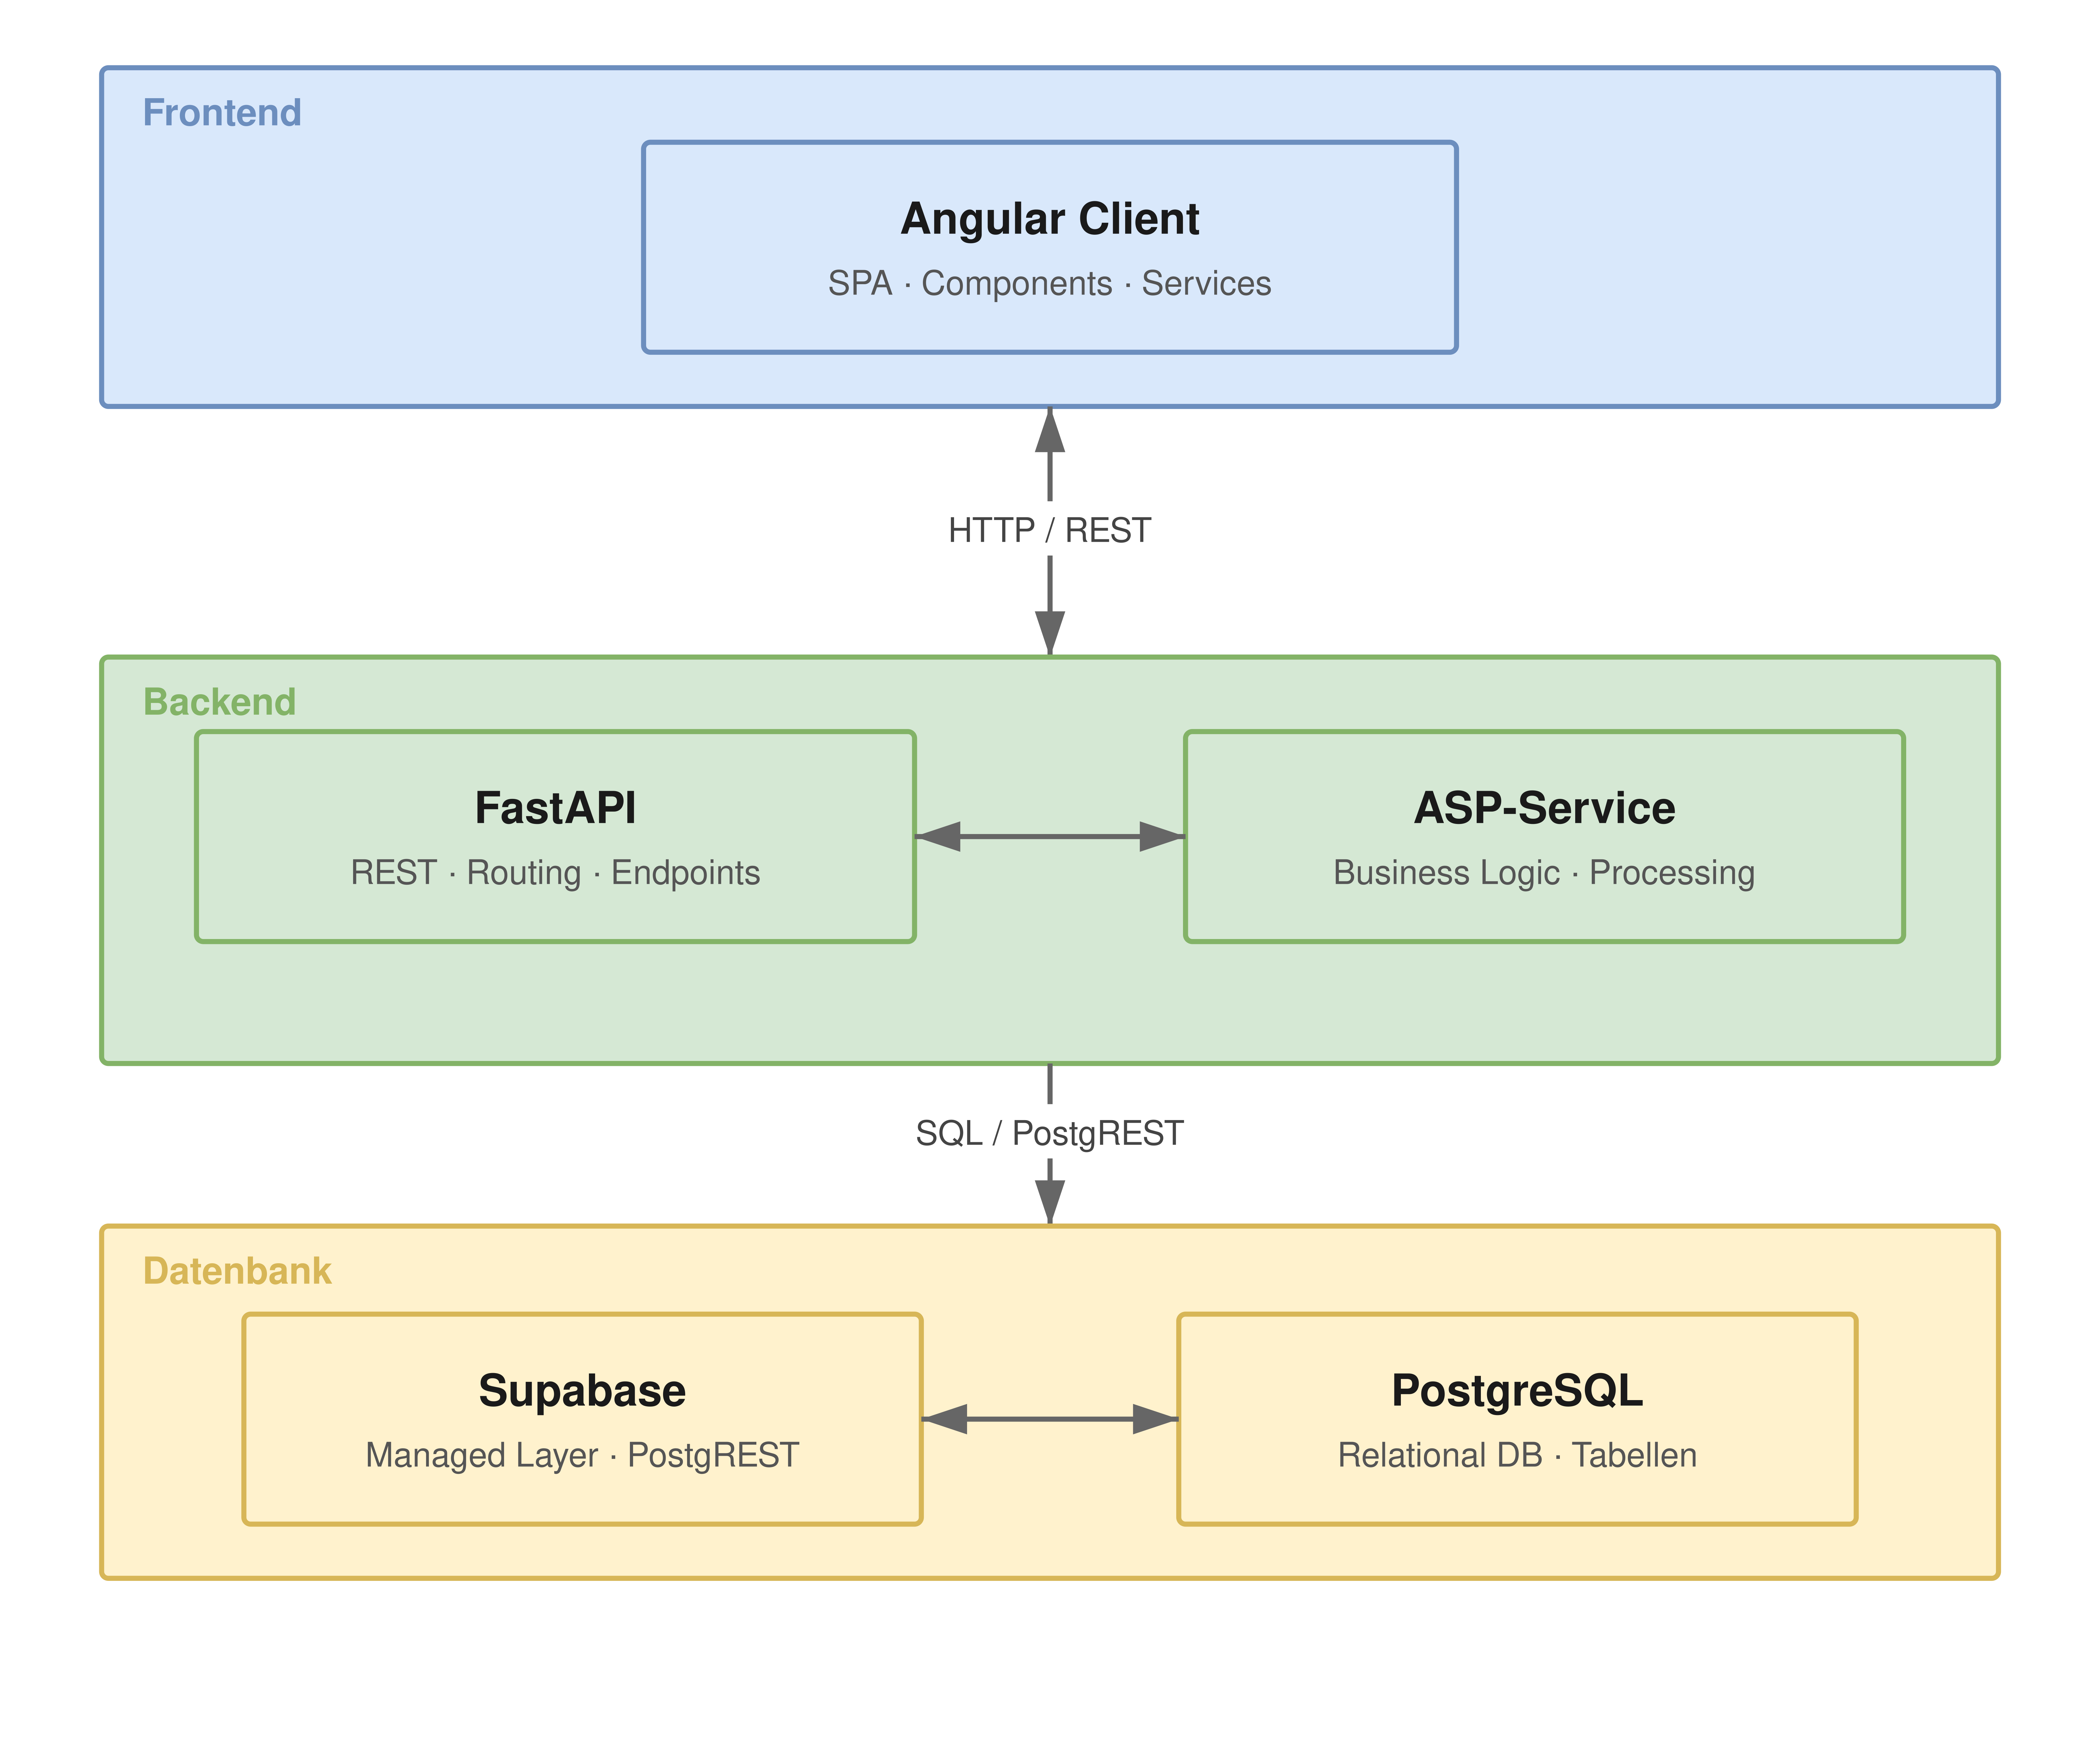
\includegraphics[width=\linewidth]{figures/architecture}
	\caption{
		Applikations-Architektur
	}\label{fig:Applikations-Architektur}
\end{figure}

Das Frontend wurde als Single-Page Application mit dem Angular Framework umgesetzt. Es stellt die Benutzeroberfläche bereit, über die Mitarbeiter, Stationen und Kompetenzen verwaltet, sowie Constraints festgelegt und Monatspläne angezeigt werden können. Die Kommunikation mit dem Backend erfolgt ausschließlich über HTTP-REST-Schnittstellen.
Das Backend ist in Python mit FastAPI realisiert und übernimmt die gesamte Geschäftslogik der Anwendung. Es stellt REST-Endpunkte bereit und verarbeitet eingehende Anfragen. Ein zentraler Bestandteil des Backends ist der ASP-Service. Dieser Service ist für die Berechnung der Monatspläne unter Berücksichtigung der definierten Hard und Soft Constraints verantwortlich.
Als Datenbankschicht wird Supabase eingesetzt, eine Open-Source-Plattform, die auf PostgreSQL aufbaut. Supabase stellt neben der relationalen Datenbank auch eine PostgREST-Schnittstelle bereit, über die das Backend direkt auf die Datenbankressourcen zugreifen kann.

\section{Datenmodell}

Das Datenmodell bildet die Grundlage für die Speicherung und Verwaltung der im System benötigten Informationen. Es wurde als relationales Datenbankschema umgesetzt und besteht aus mehreren Entitäten, die als Datenbanktabellen realisiert sind. Neben den zentralen Tabellen zur Abbildung von Mitarbeitenden, Kompetenzen, Stationen und Dienstplänen enthält das Modell verschiedene Assoziationstabellen zur Darstellung von Beziehungen zwischen diesen Entitäten. Die Struktur sowie die Beziehungen der einzelnen Tabellen sind in der Abbildung \ref{fig:Datenmodell} dargestellt. Im Folgenden werden die einzelnen Tabellen und ihre Zusammenhänge näher erläutert.

\subsection{Entitäten}

Die Tabelle \texttt{users} repräsentiert die Mitarbeitenden des Systems. Neben dem Primärschlüssel \texttt{id} wird der Name eines Mitarbeitenden im Attribut \texttt{name} gespeichert. Die Tabelle dient als zentraler Bezugspunkt für Qualifikations- und Zuweisungsbeziehungen.

Die Tabelle \texttt{skills} bildet die im System verfügbaren Kompetenzen ab. Jede Kompetenz wird durch eine eindeutige \texttt{id} sowie einen \texttt{name} beschrieben.

Die Tabelle \texttt{stations} modelliert die Arbeitsstationen, denen Mitarbeitende zugewiesen werden können. Das Attribut \texttt{maxAssignments} definiert die maximale Anzahl gleichzeitiger Zuweisungen pro Station und stellt somit eine wesentliche Kapazitätsbeschränkung dar.

Die Tabelle \texttt{schedules} dient der Verwaltung von Dienstplänen. Über die Attribute \texttt{year} und \texttt{month} können Dienstpläne zeitlich eingeordnet werden. Das Attribut \texttt{is\_loaded} speichert, welcher Dienstplan aktuell im Kalender geladen ist.

\subsection{Assoziationstabellen}

Die Tabelle \texttt{user\_skills} stellt die Zuordnung zwischen den Tabellen \texttt{users} und \texttt{skills} her. Dadurch kann gespeichert werden, über welche Qualifikationen ein Benutzer verfügt, wobei einem Benutzer mehrere Fähigkeiten zugewiesen sein können und eine Fähigkeit wiederum mehreren Benutzern zugeordnet werden kann. Die Tabelle besteht ausschließlich aus den beiden Fremdschlüsseln \texttt{user\_id} und \texttt{skill\_id}.

Die Tabelle \texttt{station\_skills} definiert die für eine Station erforderlichen Qualifikationen und stellt die Verbindung zwischen den Tabellen \texttt{stations} und \texttt{skills} her. Eine Station kann dabei über mehrere notwendige Qualifikationen verfügen. Diese Informationen ermöglichen anschließend den Abgleich zwischen den Fähigkeiten der Benutzer und den Anforderungen der jeweiligen Stationen.

Die Tabelle \texttt{station\_assignments} stellt die zentrale Verknüpfung des Datenmodells dar. Sie ordnet für ein bestimmtes Datum (\texttt{date}) eine Station (\texttt{station\_id}) einem Benutzer (\texttt{user\_id}) sowie einem Dienstplan (\texttt{schedule\_id}) zu. Das Attribut \texttt{user\_id} ist optional, sodass auch Zuweisungen ohne konkreten Benutzer gespeichert werden können. Dies ermöglicht die Abbildung von Platzhalterzuweisungen für den Fall, dass einem Dienstplan nicht für jede Station unmittelbar ein Mitarbeiter zugeordnet werden kann. Der \textit{Unique Constraint} auf den Spalten \texttt{schedule\_id}, \texttt{date} und \texttt{user\_id} stellt dabei sicher, dass ein Benutzer eines Dienstplans pro Tag nur einer einzigen Station zugewiesen werden kann.
\begin{figure}[h]
	\centering
	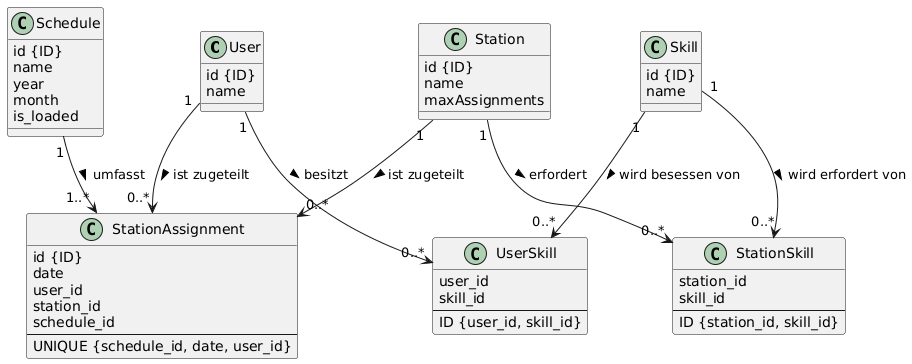
\includegraphics[width=\linewidth]{figures/datenmodell_plantuml}
	\caption{
		Datenmodell
	}\label{fig:Datenmodell}
\end{figure}

%% 
%%%%%%%%%%%%%%%%%%%%%%%%%%%%%%%%%%%%%%%%%%%%%%%%%%%%%%%%%%%%%%%%%%%%%%%%%%%%%%%%

	\input{mainmatter/05-rest}
	%%%%%%%%%%%%%%%%%%%%%%%%%%%%%%%%%%%%%%%%%%%%%%%%%%%%%%%%%%%%%%%%%%%%%%%%%%%%%%%%
%% 

\chapter{ASP-Logik}
In diesem Kapitel wird genauer auf die ASP-Logik und die Generierung der Dienstpläne eingegagen.
\section{Fakten-Generierung}
Die Fakten-Generierung stellt die Verbindung zwischen der relationalen Datenbank und der ASP-Wissensbasis dar. Damit Clingo einen Dienstplan berechnen kann, müssen die benötigten Informationen zunächst in Form von ASP-Fakten bereitgestellt werden. Dafür werden die aus der Datenbank geladenen ORM-Objekte in der Funktion \texttt{\_build\_base\_facts} in entsprechende Fakten umgewandelt.

Für jeden Benutzer wird dabei ein \texttt{user}-Fakt erzeugt. Zusätzlich wird für jede vorhandene Kompetenz ein \texttt{has\_skill}-Fakt erstellt. Für Stationen werden ebenfalls Fakten generiert, darunter \texttt{station}, \texttt{max\_assignments} zur maximalen Anzahl an Zuweisungen sowie \texttt{requires} für benötigte Kompetenzen.

Die zu planenden Arbeitstage werden als \texttt{day}-Fakten an Clingo übergeben. Wochenenden werden dabei bereits vorher durch die Funktion \texttt{get\_weekdays} herausgefiltert. Zusätzlich werden benutzerspezifische Einschränkungen als Fakten festgelegt. Dazu zählen beispielsweise maximale oder minimale Arbeitstage pro Monat (\texttt{max\_days}, \texttt{min\_days}), fixe Arbeitstage (\texttt{fixed\_day}) oder gesperrte Tage (\texttt{blocked\_day}).

Im Folgenden wird beispielhaft ein Ausschnitt der generierten Basisfakten für ein \textit{Scheduling} gezeigt. 

\begin{lstlisting}[caption={Beispiel generierter Basisfakten},label={lst}]
	user(1597).
	has_skill(1597, 23).
	has_skill(1597, 24).
	
	user(1598).
	has_skill(1598, 22).
	has_skill(1598, 25).
	
	station(865).
	max_assignments(865, 3).
	requires(865, 22).
	requires(865, 23).
	
	station(866).
	max_assignments(866, 3).
	requires(866, 24).
	
	day(1).
	day(4).
	day(5).
	
	exact_days(1597, 21).
	exact_days(1598, 21).
\end{lstlisting}
In diesem Beispiel werden zwei Benutzer, deren Kompetenzen, Stationen mit den benötigten Kompetenzen sowie Arbeitstage und Constraints als Fakten definiert. Auf Basis dieser Informationen kann Clingo anschließend gültige Dienstpläne berechnen.

\section{Regelwerk}
%First Draft%
Das Regelwerk für die initiale Planerstellung ist in der Datei \texttt{rules.lp} 
definiert. Die Grundlage bildet die Bestimmung der \textit{Eligibility}: Ein 
Benutzer gilt als qualifiziert für eine Station (\texttt{eligible/2}), wenn er 
alle erforderlichen Fähigkeiten besitzt, also kein \texttt{requires/2}-Fakt 
existiert, dem kein entsprechendes \texttt{has\_skill/2}-Fakt gegenübersteht. 
Daraus wird \texttt{eligible\_day/3} abgeleitet, welches zusätzlich gesperrte 
Tage ausschließt. Der \textit{Entscheidungsraum} wird durch eine \textit{Choice 
	Rule} definiert, die Clingo erlaubt, Benutzern Stationen an bestimmten Tagen 
zuzuweisen, wobei pro Station und Tag maximal \texttt{Max} Benutzer zugewiesen 
werden dürfen. Die \textit{harten Constraints} erzwingen, dass kein Benutzer an 
zwei Stationen gleichzeitig eingeteilt wird, dass gesperrte Tage nicht belegt 
werden, und dass benutzerspezifische Einschränkungen wie \texttt{max\_days/2}, 
\texttt{min\_days/2} sowie \texttt{exact\_days/2} eingehalten werden. Fixe 
Arbeitstage werden über \texttt{fixed\_day/2} als harte Bedingung erzwungen, 
sodass bestimmte Benutzer an vordefinierten Tagen zwingend eingeteilt sind. 
Die \textit{Optimierung} minimiert unbesetzte Stationen über eine 
\texttt{\#minimize}-Direktive, die Clingo anweist, die Anzahl der Tage, an 
denen eine Station ohne Besetzung bleibt, so gering wie möglich zu halten. 
Die Regelstruktur für das Rescheduling folgt einem ähnlichen Prinzip, wird 
jedoch in Abschnitt~\ref{sec:rescheduling} gesondert behandelt.
\section{Zweiphasen-Lösungsanstz}

\section{Rescheduling-Logik}

\section{Timeout NP-hartes Problem}



%% 
%%%%%%%%%%%%%%%%%%%%%%%%%%%%%%%%%%%%%%%%%%%%%%%%%%%%%%%%%%%%%%%%%%%%%%%%%%%%%%%%

	%%%%%%%%%%%%%%%%%%%%%%%%%%%%%%%%%%%%%%%%%%%%%%%%%%%%%%%%%%%%%%%%%%%%%%%%%%%%%%%%
%% 

\chapter{Conclusio und Ausblick}

Im Rahmen dieser Bachelorarbeit wurde ein ASP-basiertes System zur automatisierten Erstellung und kurzfristigen Anpassung von Dienstplänen entwickelt und als vollständige Fullstack-Webanwendung umgesetzt. Die Arbeit zeigt, dass Answer Set Programming mit Clingo eine geeignete Grundlage für praxisnahe Planungssoftware im Gesundheitssektor darstellt. Das implementierte Rescheduling-Verfahren sowie die Möglichkeit zur vorausschauenden Berechnung von Alternativplänen erhöhen die praktische Einsetzbarkeit des Systems zusätzlich.

Dennoch unterliegt die vorliegende Arbeit einigen Einschränkungen. Die betrachtete Problemvariante beschränkt sich auf eine einheitliche Tagesschicht, was die Komplexität gegenüber Szenarien mit mehreren Schichttypen reduziert. Darüber hinaus basiert die Evaluierung ausschließlich auf manuell erstellten Testdaten, sodass eine Validierung unter realen Bedingungen noch aussteht. Bei stark wachsender Instanzgröße ist zudem zu erwarten, dass die Berechnungszeit zunimmt, was in dieser Arbeit nicht systematisch untersucht wurde.

Für zukünftige Weiterentwicklungen bieten sich mehrere Ansatzpunkte an. Eine naheliegende Erweiterung ist die Unterstützung mehrerer Schichttypen wie Früh-, Spät- und Nachtschicht, um das System für ein breiteres Spektrum an Krankenhausabteilungen nutzbar zu machen. Darüber hinaus könnte das ASP-Encoding hinsichtlich Laufzeit und Skalierbarkeit weiter optimiert werden. Auch die Erweiterung der Soft Constraints, beispielsweise um persönliche Wunschfreitage der Mitarbeitenden würde die Planungsqualität und Akzeptanz in der Praxis verbessern. Schließlich wäre die Integration und Evaluierung mit realen Krankenhausdaten ein wichtiger Schritt, um die tatsächliche Praxistauglichkeit des Systems zu validieren.




%% 
%%%%%%%%%%%%%%%%%%%%%%%%%%%%%%%%%%%%%%%%%%%%%%%%%%%%%%%%%%%%%%%%%%%%%%%%%%%%%%%%


	
	%%%%%%%%%%%%%%%%%%%%%%%%%%%%%%%%%%%%%%%%%
	%%%% Back Matter                     %%%% 
	%%%%%%%%%%%%%%%%%%%%%%%%%%%%%%%%%%%%%%%%%
	\backmatter
	\input{backmatter/misc}
	\appendix
	% !TeX root = ../MAIN.tex
% !TeX encoding = UTF-8

\chapter{Anhang A - Benutzerdokumentation}
In diesem Kapitel wird die Benutzerdokumentation vorgestellt, die die Nutzung des Systems beschreibt und den Anwender bei der Verwendung der bereitgestellten Funktionen unterstützt.

\subsection{Stammdaten anlegen}
Für die Nutzung des NSP-Solvers müssen zunächst die erforderlichen Stammdaten im System angelegt werden. Voraussetzung dafür ist, dass das Angular-Frontend und das FastAPI-Backend gestartet sind und eine Verbindung zur Datenbank besteht. Anschließend können Daten wie die Mitarbeiter, die zu besetzenden Stationen sowie die benötigten Kompetenzen angelegt werden. Für jeden Mitarbeiter wird der Name, sowie die vorhandenen Kompetenzen hinterlegt. Anschließend werden die Stationen definiert, die im Dienstplan berücksichtigt werden sollen. Auch hier wird einfach ein Name und die erforderlichen Kompetenzen festgelegt. Außerdem müssen die Kompetenzen angelegt werden, damit diese den Mitarbeitern und Stationen zugeordnet werden können. Erst wenn alle erforderlichen Stammdaten vollständig erfasst wurden, können Schichtanforderungen definiert und Dienstpläne mithilfe des NSP-Solvers erstellt werden.
Abbildung \ref{fig:user_list} zeigt die Übersichts-Liste von Mitarbeitern.

\begin{figure}[h]
	\centering
	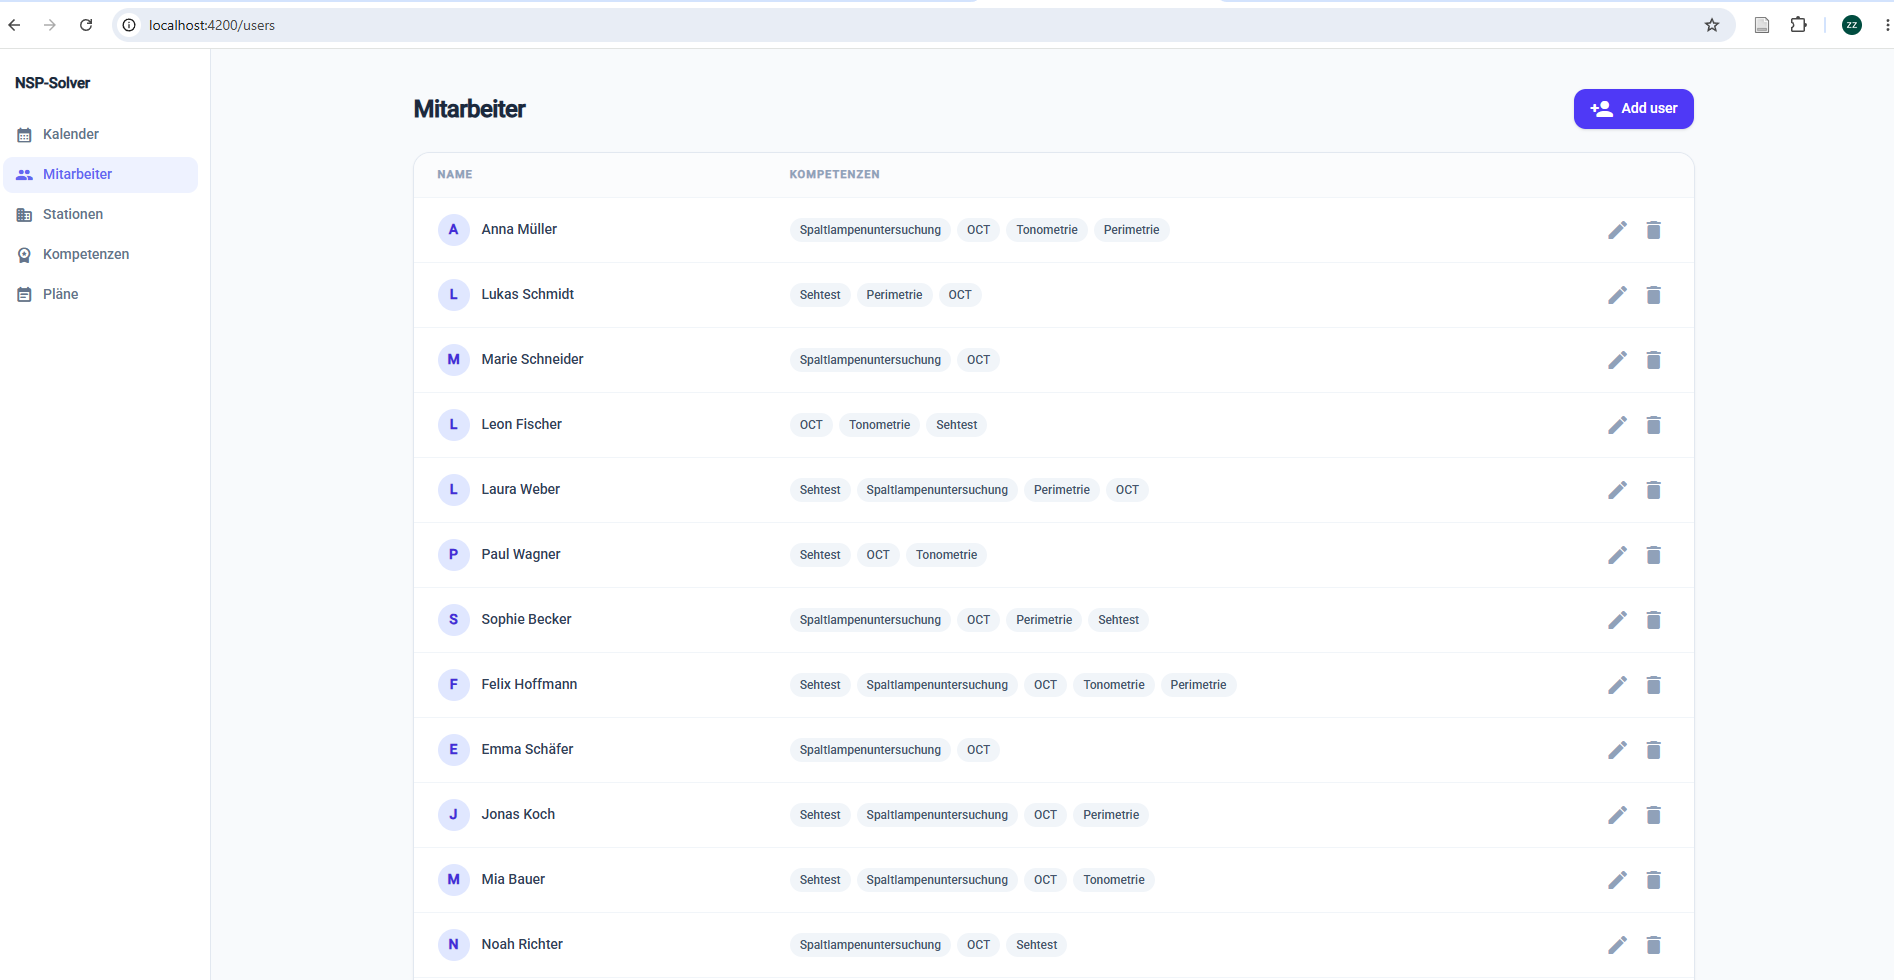
\includegraphics[width=\linewidth]{figures/user_list}
	\caption{
		Liste von Mitarbeitern
	}\label{fig:user_list}
\end{figure}

Über eine Unterseite kann man gewünschte Mitarbeiter mit den jeweiligen Kompetenzen anlegen. Die Unterseite wird in Abbildung \ref{fig:create_user} dargestellt.
\begin{figure}[h]
	\centering
	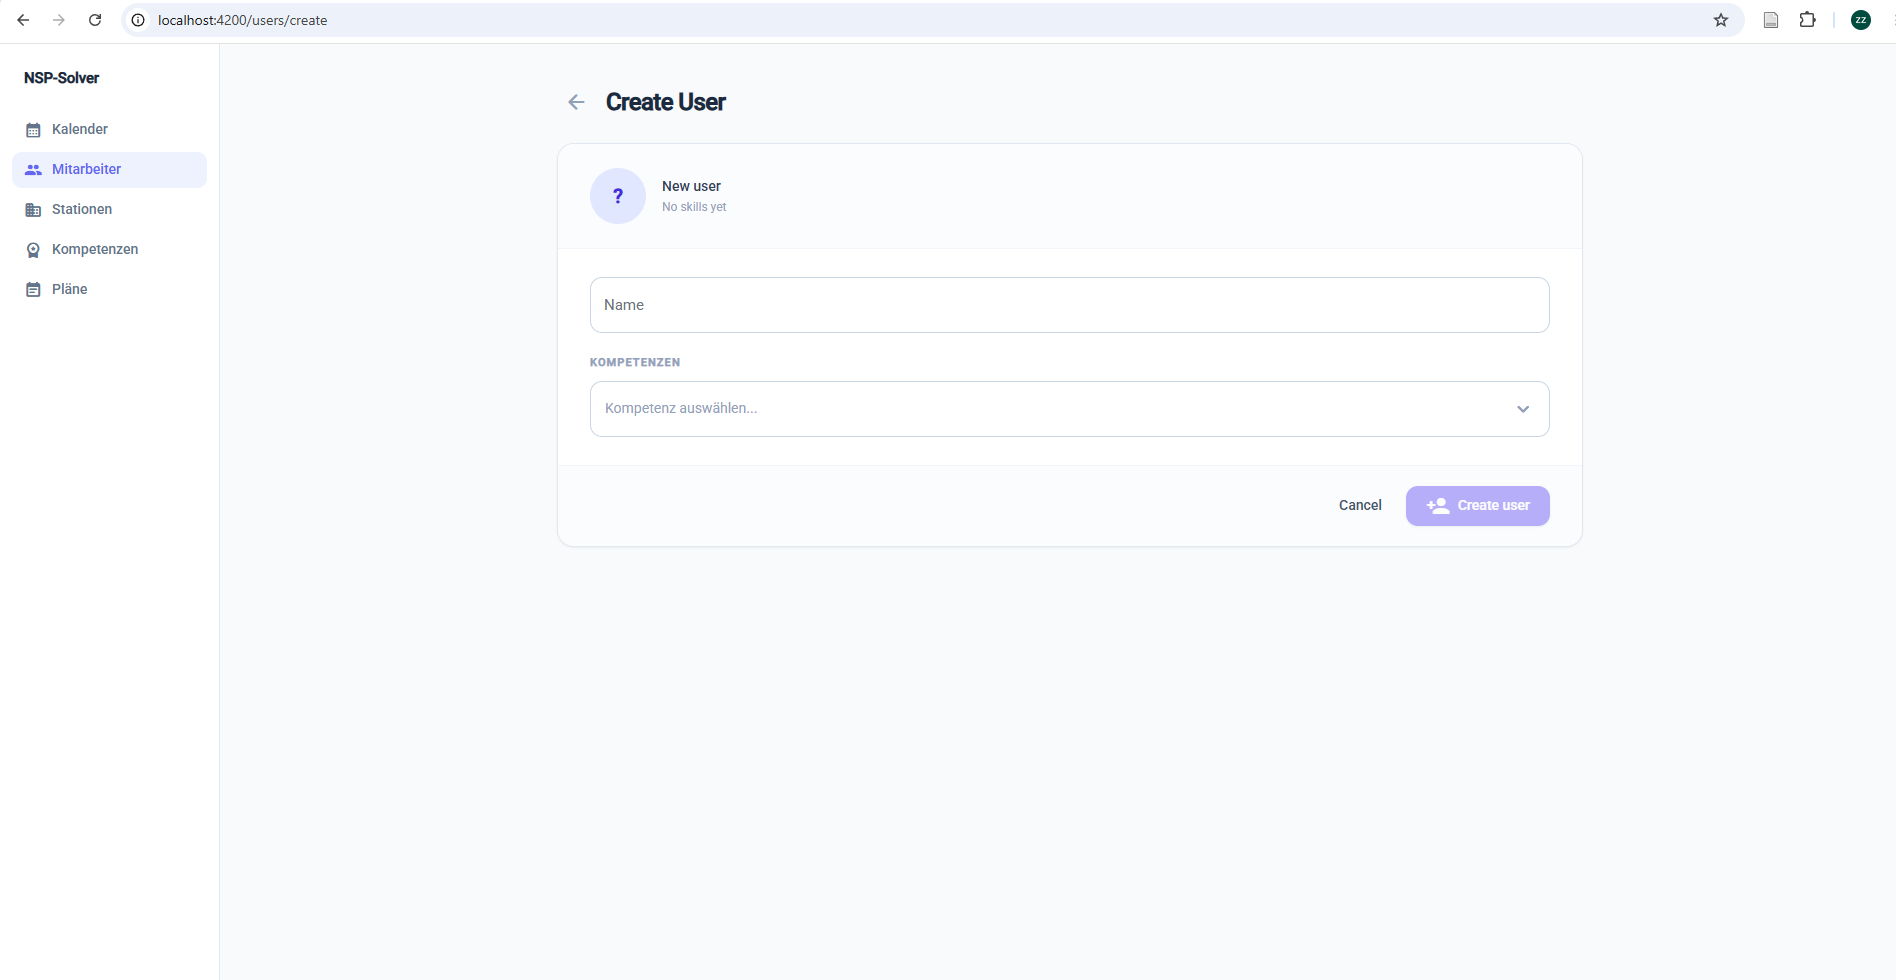
\includegraphics[width=\linewidth]{figures/create_user}
	\caption{
		Mitarbeiter erstellen
	}\label{fig:create_user}
\end{figure}

Analog dazu können auch Stationen und Kompetenzen auf den entsprechenden Unterseiten angelegt werden. \newline
Auf der Unterseite \textit{Kalendar} bekommt man eine Übersicht für den Monat. Wie die Unterseite aussieht, wird in Abbildung \ref{fig:calendar} dargestellt.

\begin{figure}[h]
	\centering
	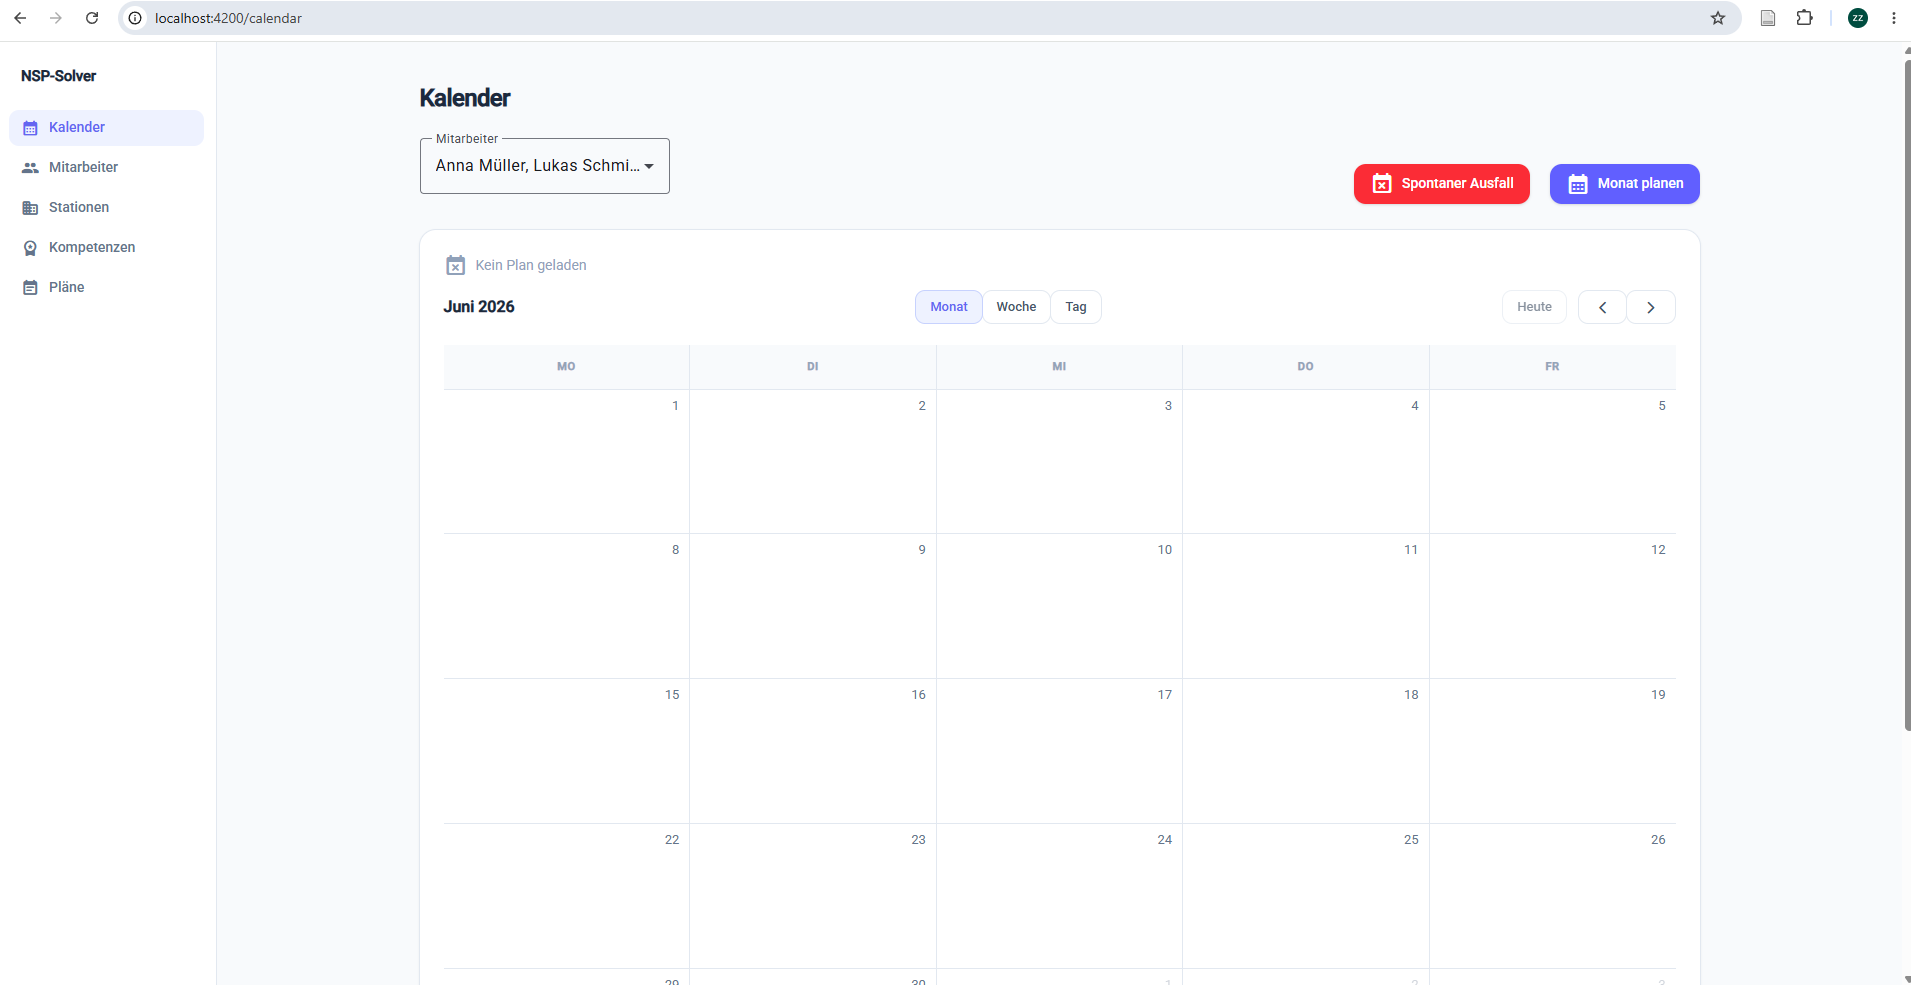
\includegraphics[width=\linewidth]{figures/calendar}
	\caption{
		Kalenderansicht
	}\label{fig:calendar}
\end{figure}

\subsection{(Re)-Scheduling}
Über den Button \textit{Monat planen} lassen sich vor dem Planungslauf individuelle Einschränkungen je Mitarbeiter festlegen. Das Dialogfenster ist in Abbildung \ref{fig:solver_dialog} dargestellt.  

\begin{figure}[h]
	\centering
	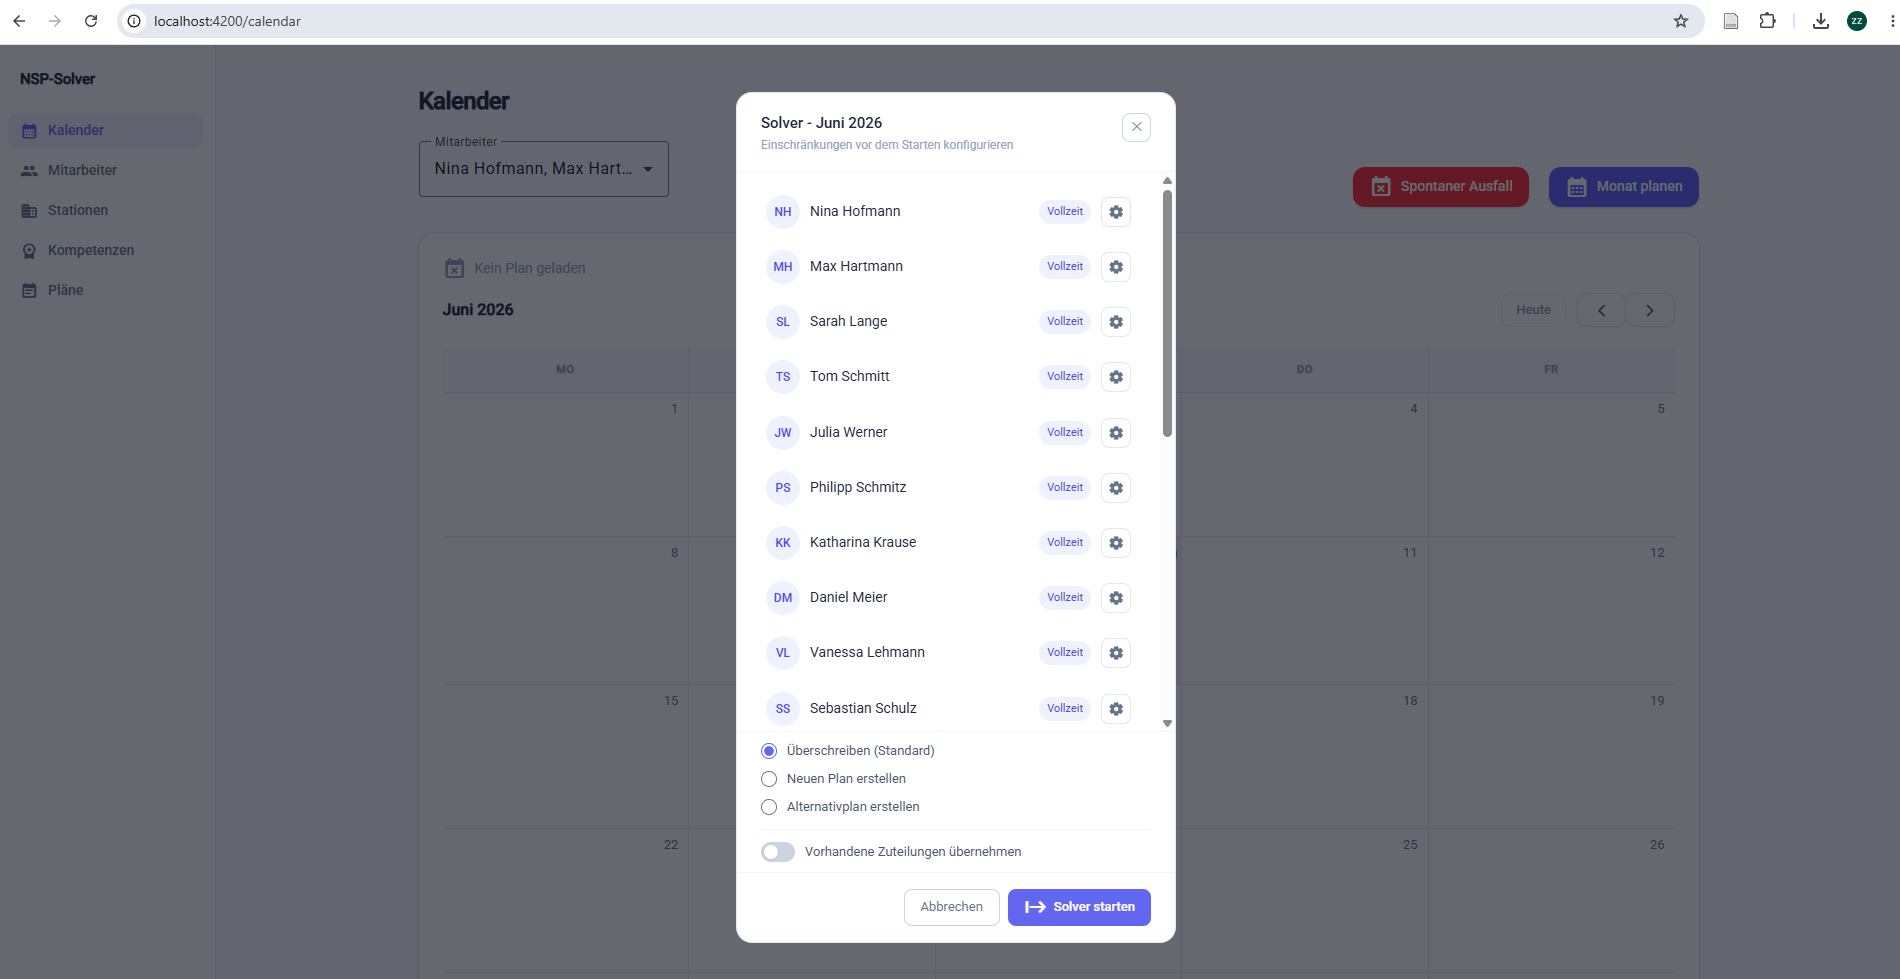
\includegraphics[width=\linewidth]{figures/solver_dialog}
	\caption{
		Solver-Dialogfenster
	}\label{fig:solver_dialog}
\end{figure}
Per Klick auf das Zahnrad-Symbol neben einem Mitarbeiter öffnet sich der Einschränkungsdialog, in dem die gewünschte Arbeitszeit für den Monat definiert wird, entweder als Vollzeit, als exakte Anzahl an Tagen oder als Spannweite. Im Abschnitt Verfügbarkeit kann anschließend über den Kalender angegeben werden, an welchen Tagen ein Mitarbeiter fix eingeplant werden soll oder nicht verfügbar ist. Nach dem Speichern der Einschränkungen stehen im Solver-Dialog außerdem drei Modi zur Auswahl: Vorhandene Zuteilungen übernehmen, Neuen Plan erstellen sowie Alternativpläne. Mit einem Klick auf \textit{Solver starten} wird die Planung unter Berücksichtigung aller konfigurierten Vorgaben ausgeführt. Das Dialogfenster für Einschränkungen wird in Abbildung \ref{fig:constraint_dialog} grafisch veranschaulicht.
\begin{figure}[h]
	\centering
	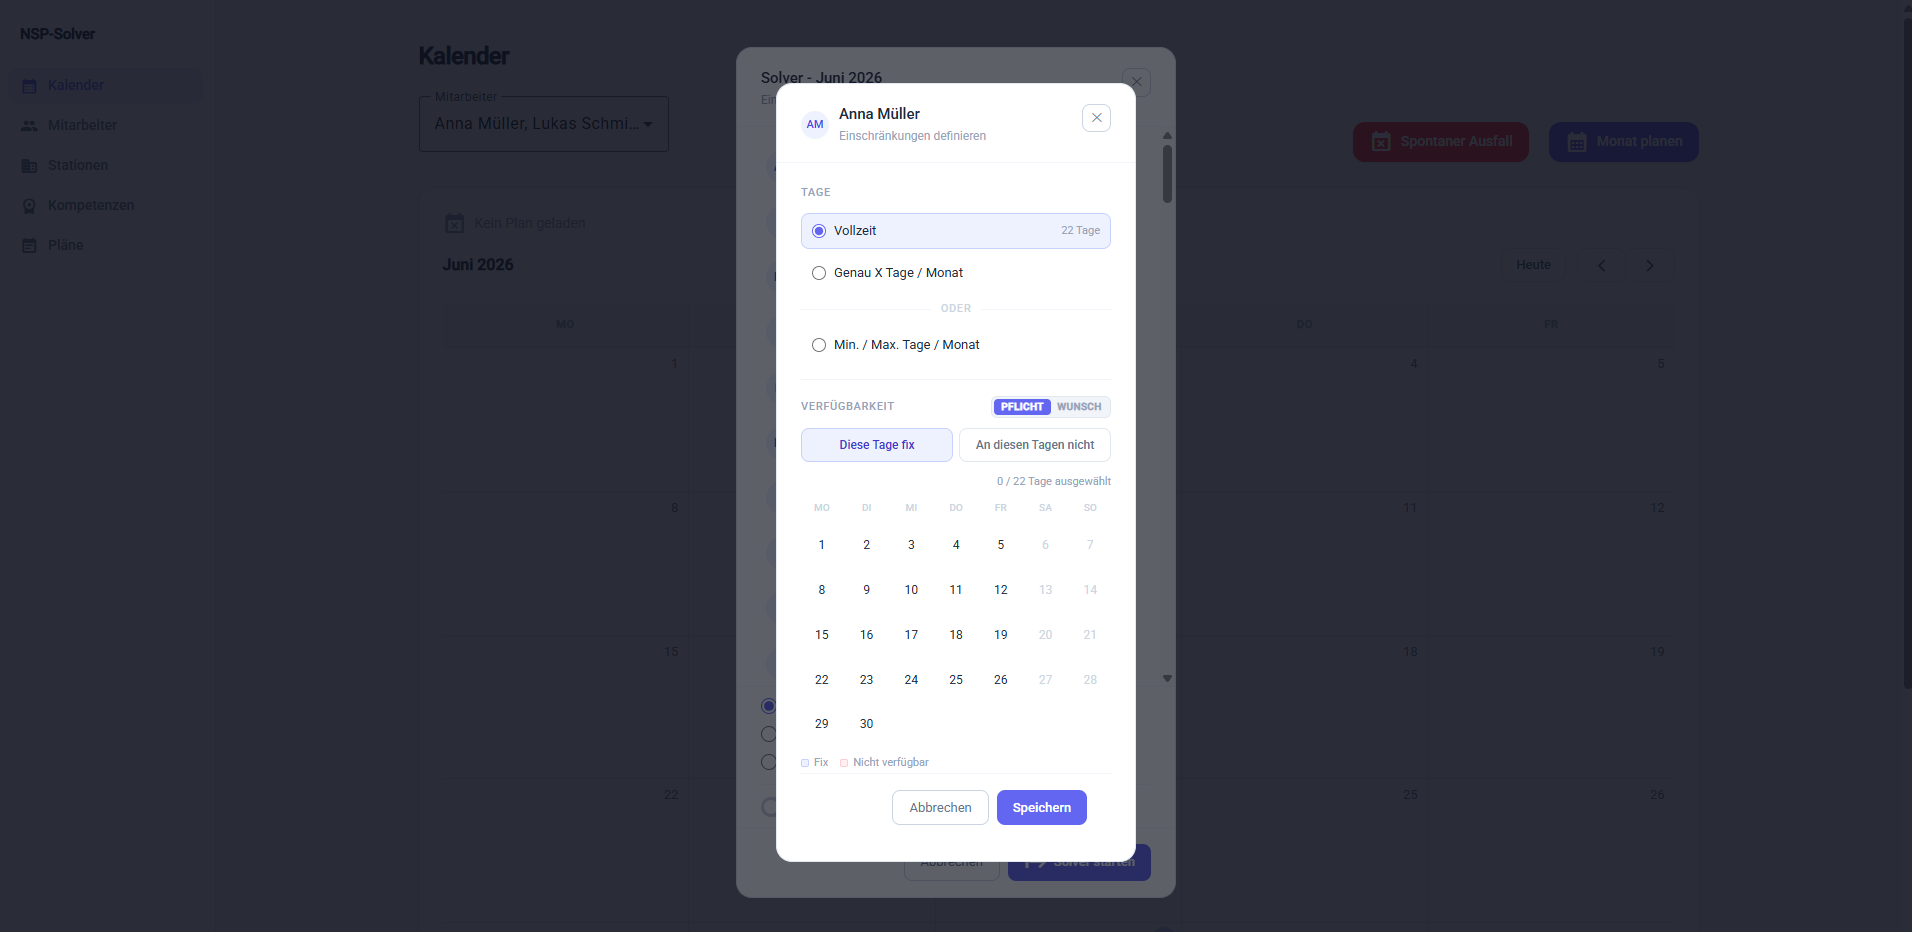
\includegraphics[width=\linewidth]{figures/constraint_dialog}
	\caption{
		Einschränkungs-Dialogfenster
	}\label{fig:constraint_dialog}
\end{figure}

Nach erfolgreichem Planungslauf werden die Zuteilungen direkt im Kalender angezeigt. Wie in Abbildung \ref{fig:calendar_full} ersichtlich, erscheinen pro Tag die zugeteilten Mitarbeiter als farbige Chips im jeweiligen Kalenderfeld.

\begin{figure}[H]
	\centering
	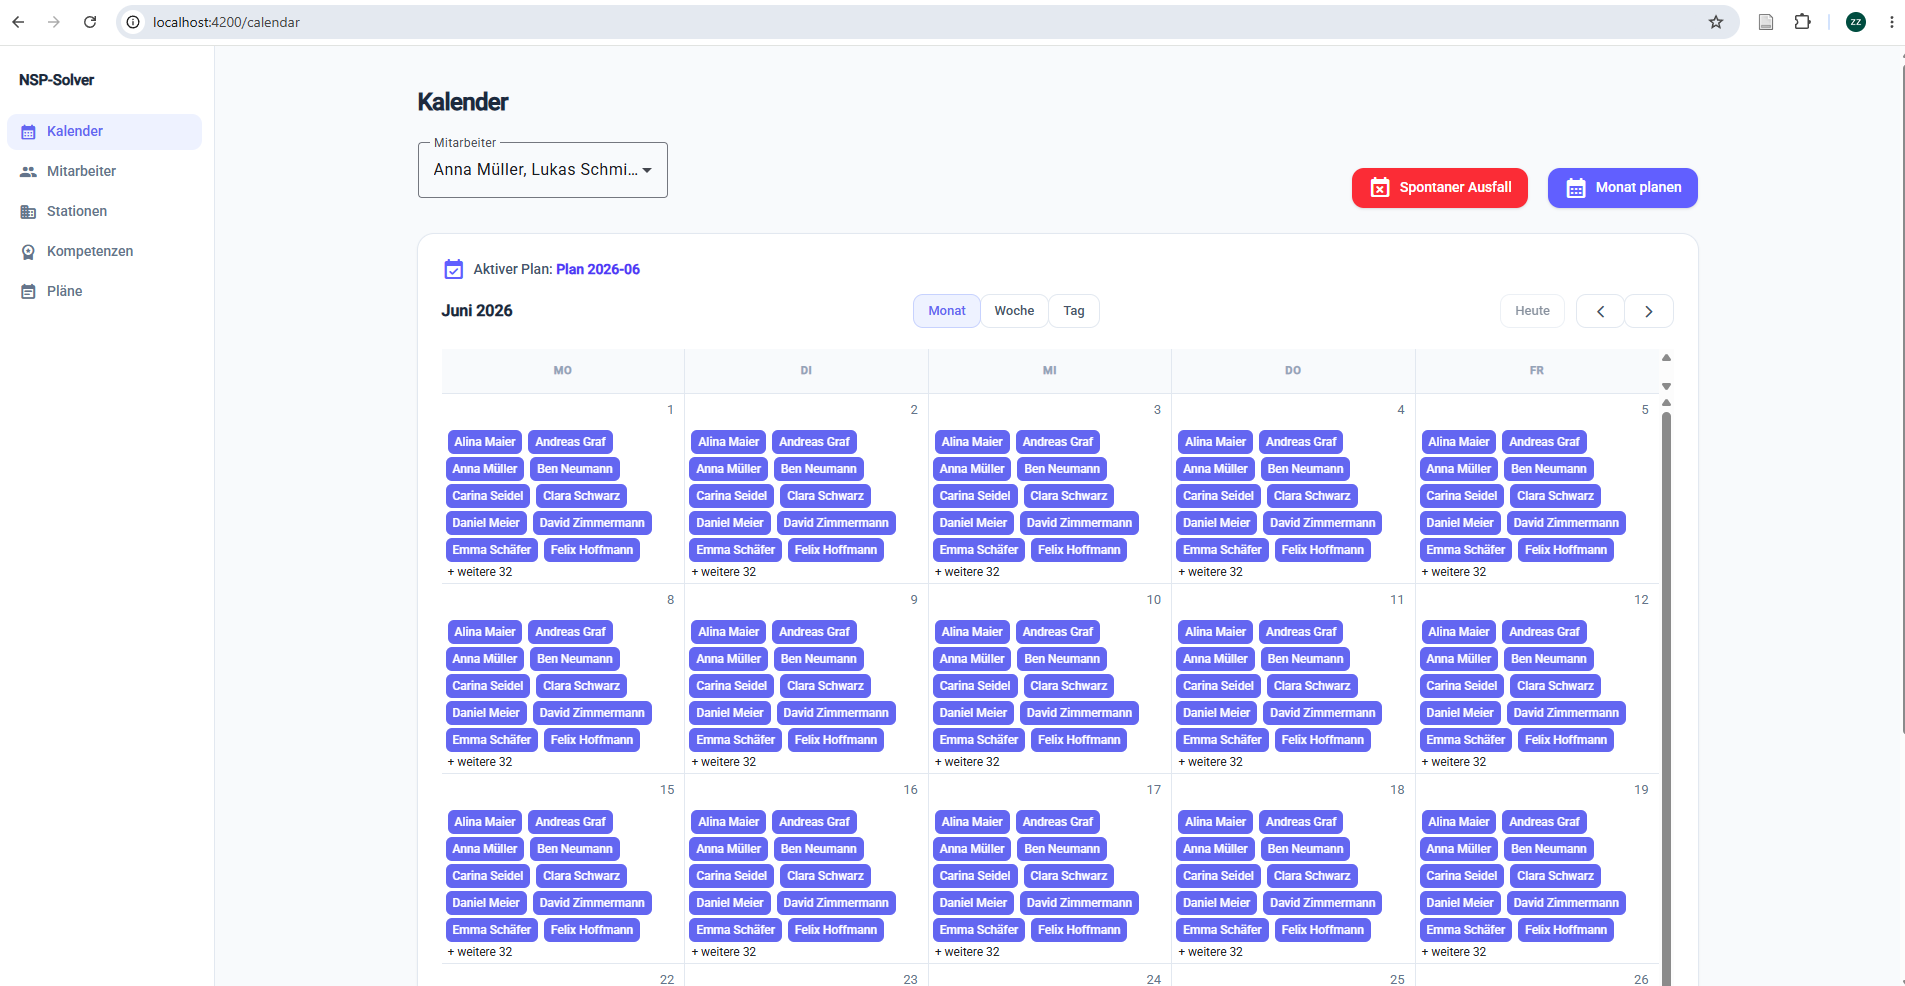
\includegraphics[width=\linewidth]{figures/calendar_full}
	\caption{
		Monatsübersicht mit Zuteilungen
	}\label{fig:calendar_full}
\end{figure}

 Über einen Klick auf einen beliebigen Tag gelangt man zur Tages-Detailansicht, in der, wie in Abbildung \ref{fig:day_detail} dargestellt, alle Stationen des jeweiligen Tages tabellarisch aufgelistet sind. Zu jeder Station ist der aktuelle Besetzungsstand sowie die namentliche Zuteilung der Mitarbeiter ersichtlich. Die Zuteilungen können dort bei Bedarf auch manuell über das Dropdown-Menü angepasst werden.
 
 \begin{figure}[H]
 	\centering
 	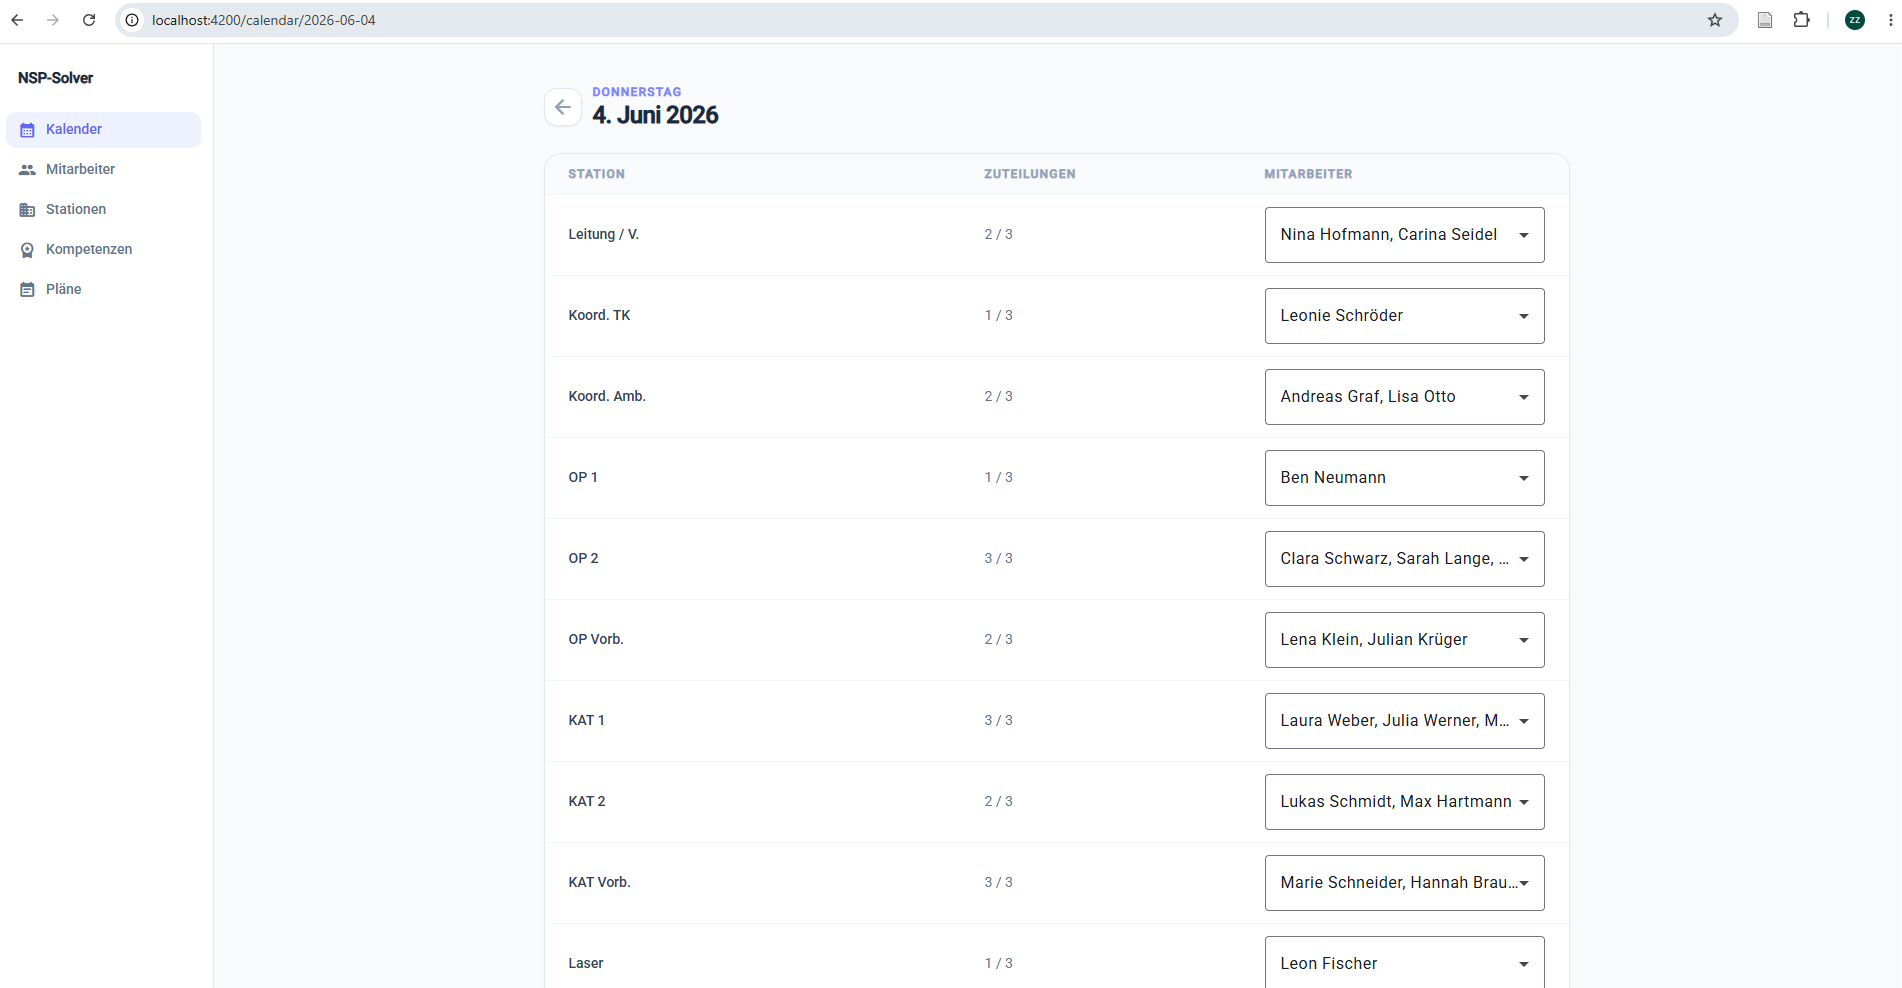
\includegraphics[width=\linewidth]{figures/day_detail}
 	\caption{
 		Monatsübersicht mit Zuteilungen
 	}\label{fig:day_detail}
 \end{figure}
 
 Fällt ein Mitarbeiter kurzfristig aus, kann über den Button \textit{Spontaner Ausfall} in der Kalenderansicht eine gezielte Umplanung ausgeführt werden. Wie in Abbildung \ref{fig:reschedule_dialog} ersichtlich, öffnet sich dabei ein Dialog, in dem für jeden Mitarbeiter ein Ausfall erfasst werden kann.
 
   \begin{figure}[H]
 	\centering
 	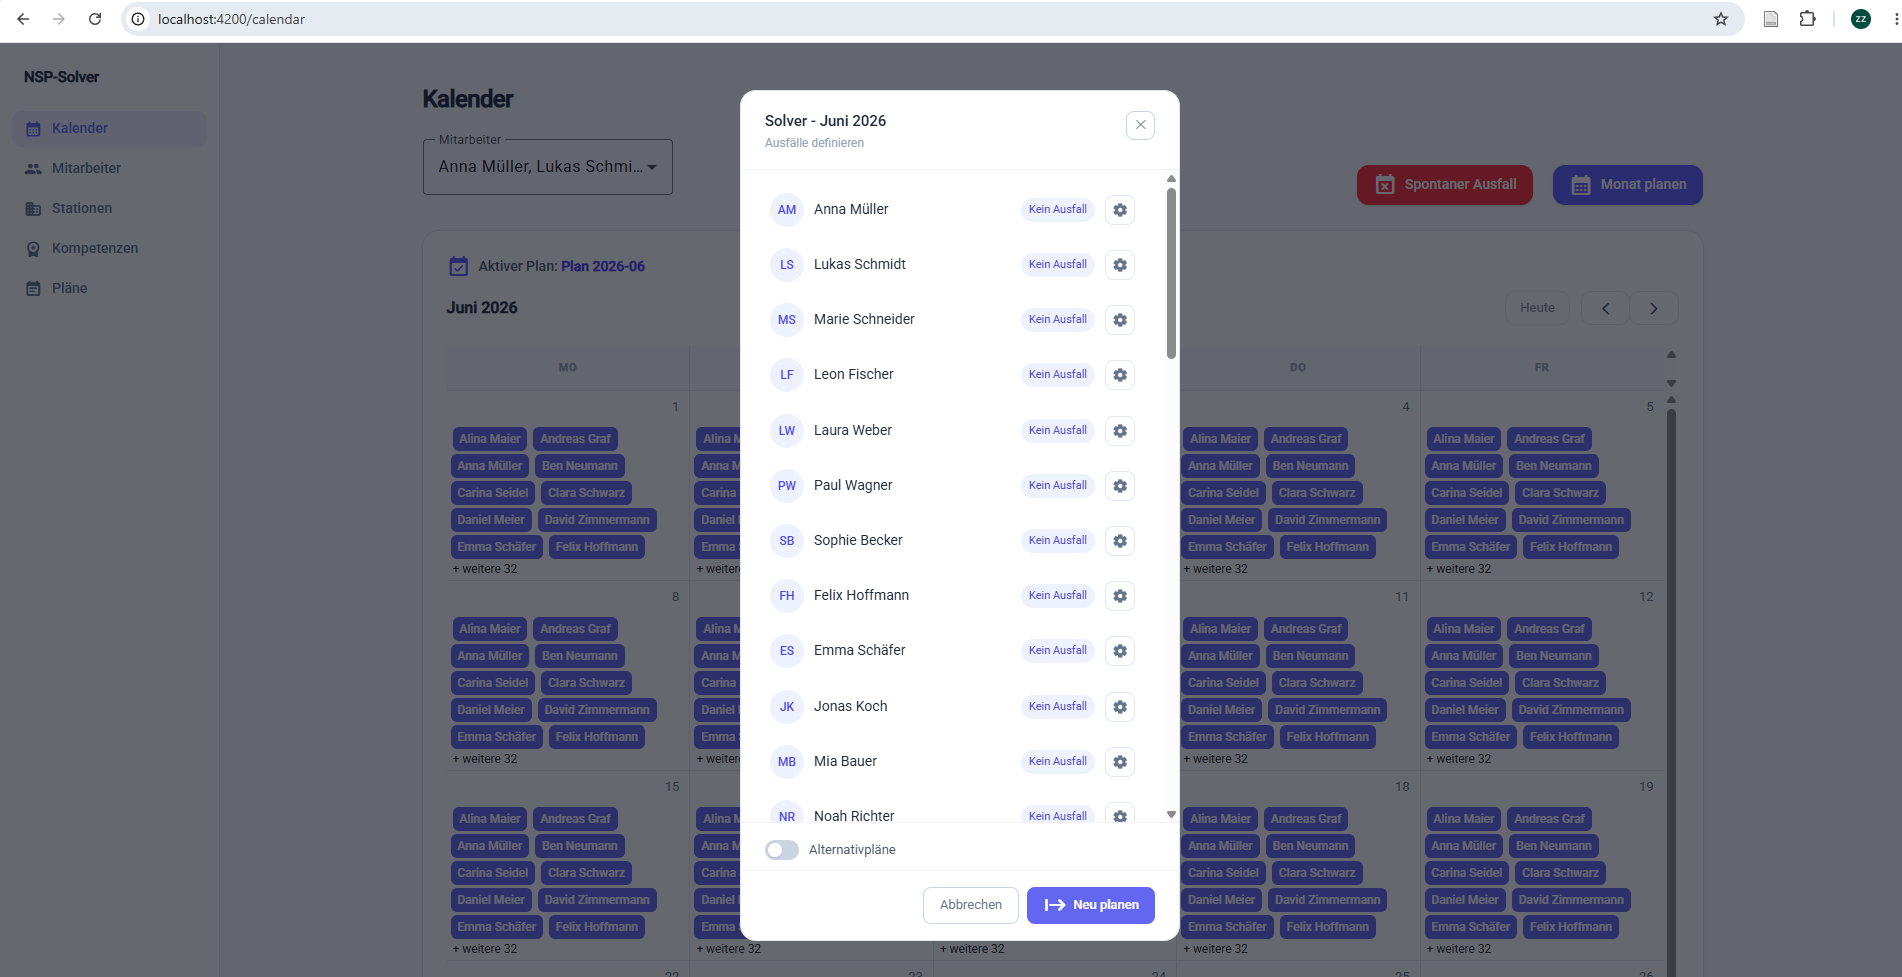
\includegraphics[width=\linewidth]{figures/reschedule_dialog}
 	\caption{
 		Reschedule-Dialogfenster
 	}\label{fig:reschedule_dialog}
 \end{figure}
 
  Per Klick auf das Zahnrad-Symbol neben einem Mitarbeiter lässt sich, wie in Abbildung \ref{fig:reschedule_constraint_dialog} dargestellt, ein Kalender öffnen, in dem die betroffenen Tage als nicht verfügbar markiert werden können. Optional kann über den Alternativpläne-Toggle gesteuert werden, ob zusätzliche Planvarianten generiert werden sollen. 
  
   \begin{figure}[H]
	\centering
	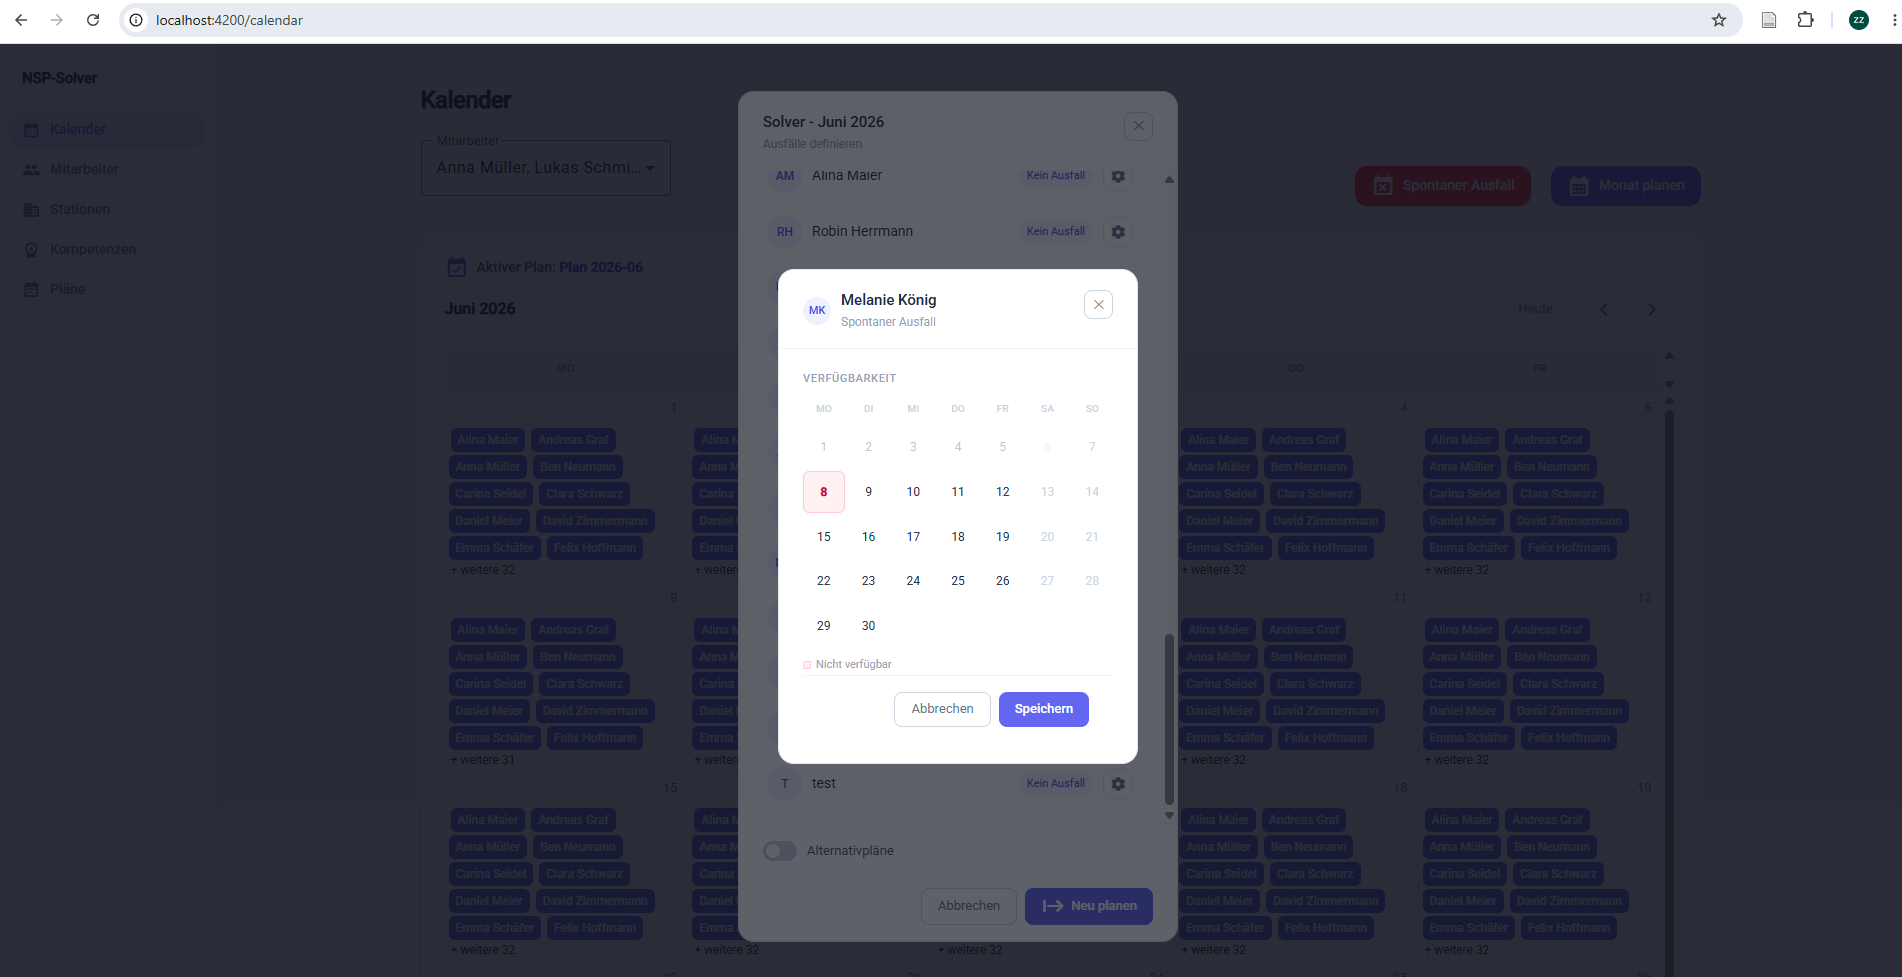
\includegraphics[width=\linewidth]{figures/reschedule_constraint_dialog}
	\caption{
		Reschedule-Dialogfenster - Einschränkungen
	}\label{fig:reschedule_constraint_dialog}
\end{figure}
  Nach dem Start der Umplanung mit \textit{Neu planen} aktualisiert der Solver den bestehenden Plan unter Berücksichtigung der neu definierten Ausfälle. Das Ergebnis wird anschließend in einem Zusammenfassungsdialog angezeigt, wie in Abbildung \ref{fig:reschedule_result} zu sehen, der übersichtlich auflistet, welche Zuteilungen entfernt und welche neu hinzugefügt wurden.

   \begin{figure}[H]
 	\centering
 	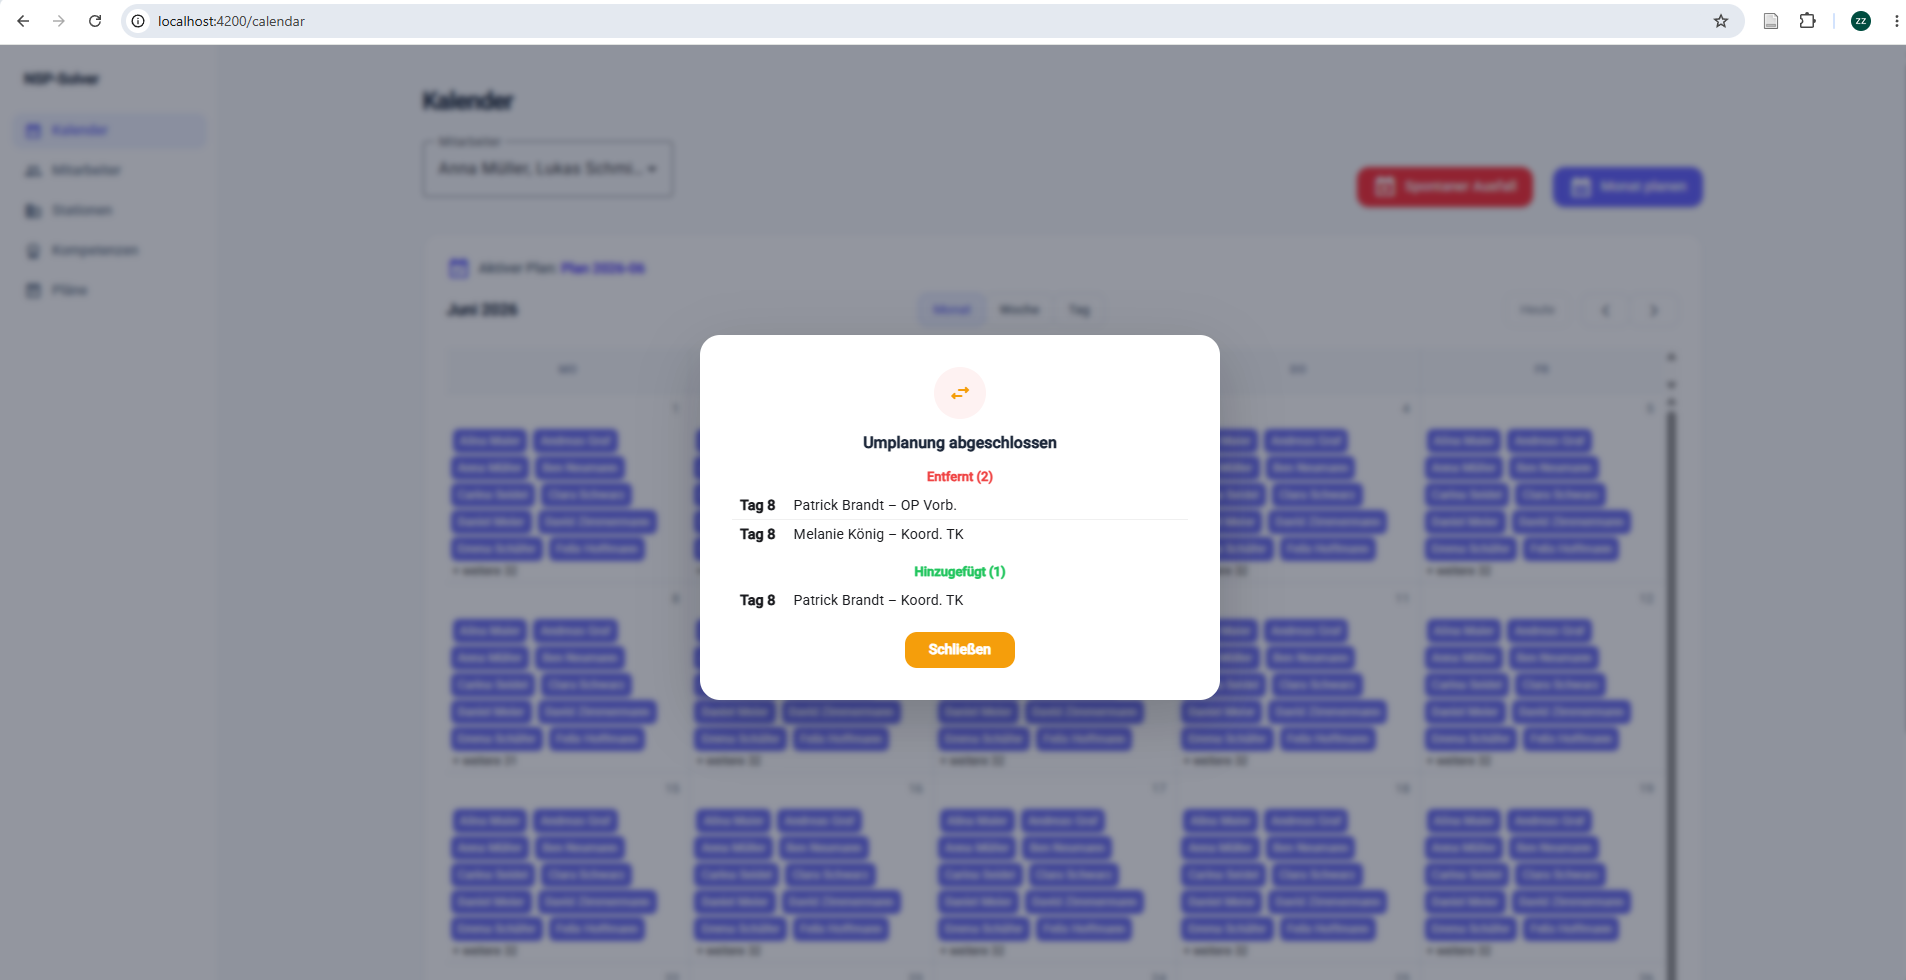
\includegraphics[width=\linewidth]{figures/reschedule_result}
 	\caption{
 		Reschedule-Ergebnis
 	}\label{fig:reschedule_result}
 \end{figure}
 
 





\end{document}